%%% Hlavní soubor. Zde se definují základní parametry a odkazuje se na ostatní části. %%%

%% Verze pro jednostranný tisk:
% Okraje: levý 40mm, pravý 25mm, horní a dolní 25mm
% (ale pozor, LaTeX si sám přidává 1in)
\documentclass[12pt,a4paper]{report}
\setlength\textwidth{145mm}
\setlength\textheight{247mm}
\setlength\oddsidemargin{15mm}
\setlength\evensidemargin{15mm}
\setlength\topmargin{0mm}
\setlength\headsep{0mm}
\setlength\headheight{0mm}
% \openright zařídí, aby následující text začínal na pravé straně knihy
\let\openright=\clearpage

%% Pokud tiskneme oboustranně:
% \documentclass[12pt,a4paper,twoside,openright]{report}
% \setlength\textwidth{145mm}
% \setlength\textheight{247mm}
% \setlength\oddsidemargin{14.2mm}
% \setlength\evensidemargin{0mm}
% \setlength\topmargin{0mm}
% \setlength\headsep{0mm}
% \setlength\headheight{0mm}
% \let\openright=\cleardoublepage

%% Vytváříme PDF/A-2u
\usepackage[a-2u]{pdfx}

%% Přepneme na českou sazbu a fonty Latin Modern
\usepackage[czech]{babel}
\usepackage{lmodern}
\usepackage[T1]{fontenc}
\usepackage{textcomp}

%% Použité kódování znaků: obvykle latin2, cp1250 nebo utf8:
\usepackage[utf8]{inputenc}

%%% Další užitečné balíčky (jsou součástí běžných distribucí LaTeXu)
\usepackage{amsmath}        % rozšíření pro sazbu matematiky
\usepackage{amsfonts}       % matematické fonty
\usepackage{amsthm}         % sazba vět, definic apod.
\usepackage{bbding}         % balíček s nejrůznějšími symboly
			    			% (čtverečky, hvězdičky, tužtičky, nůžtičky, ...)
\usepackage{bm}             % tučné symboly (příkaz \bm)
\usepackage{graphicx}       % vkládání obrázků
\usepackage{fancyvrb}       % vylepšené prostředí pro strojové písmo
\usepackage{indentfirst}    % zavede odsazení 1. odstavce kapitoly
\usepackage{natbib}         % zajišťuje možnost odkazovat na literaturu
							% stylem AUTOR (ROK), resp. AUTOR [ČÍSLO]
\usepackage[nottoc]{tocbibind} % zajistí přidání seznamu literatury,
                            % obrázků a tabulek do obsahu
\usepackage{icomma}         % inteligetní čárka v matematickém módu
\usepackage{dcolumn}        % lepší zarovnání sloupců v tabulkách
\usepackage{booktabs}       % lepší vodorovné linky v tabulkách
\usepackage{paralist}       % lepší enumerate a itemize
\usepackage{xcolor}         % barevná sazba

\usepackage{float}			% umístění figure bloků
\usepackage{wrapfig}        % obrázek plující vedle textu
\usepackage{multicol}       % sloupečky
\usepackage{listings}		% highlighting kódu
\usepackage{makecell}		% víceřádková buňka v tabulce


\usepackage[font=scriptsize, skip=1pt]{caption}		% pro seznam obrázku a tabulek
\DeclareCaptionLabelSeparator{bar}{\space\textbar\space}
\captionsetup{labelsep=bar}
\addto\captionsczech{\renewcommand{\figurename}{Obr.}}


%\usepackage[light,scaled=0.85]{roboto-mono}




% Zapne černé "slimáky" na koncích řádků, které přetekly, abychom si
% jich lépe všimli.
% \overfullrule=3mm % vypnout pro produkci TODO

%%% Údaje o práci

% Název práce v jazyce práce (přesně podle zadání)
\def\NazevPrace{Softwarové řešení digitálních archivů}

% Název práce v angličtině
\def\NazevPraceEN{Software solution for digital archives}

% Jméno autora
\def\AutorPrace{David Nápravník}

% Rok odevzdání
\def\RokOdevzdani{2021}

% Název katedry nebo ústavu, kde byla práce oficiálně zadána
% (dle Organizační struktury MFF UK, případně plný název pracoviště mimo MFF)
\def\Katedra{Katedra teoretické informatiky a matematické logiky}
\def\KatedraEN{Department of Theoretical Computer Science and Mathematical Logic}

% Jedná se o katedru (department) nebo o ústav (institute)?
\def\TypPracoviste{Katedra}
\def\TypPracovisteEN{Department}

% Vedoucí práce: Jméno a příjmení s~tituly
\def\Vedouci{Mgr. Kateřina Macková}

% Pracoviště vedoucího (opět dle Organizační struktury MFF)
\def\KatedraVedouciho{Katedra teoretické informatiky a matematické logiky}
\def\KatedraVedoucihoEN{Department of Theoretical Computer Science and Mathematical Logic}

% Studijní program a obor
\def\StudijniProgram{Informatika (B1801)}
\def\StudijniObor{IPSS (1801R048)}

% Nepovinné poděkování (vedoucímu práce, konzultantovi, tomu, kdo
% zapůjčil software, literaturu apod.)
\def\Podekovani{
	\section*{Poděkování}
	Chtěl bych poděkovat Mgr. Kateřině Mackové za odborné vedení práce a
	cenné rady, které mi pomohly tuto práci zkompletovat.
	Anně Yaghobové a Monice Bošániové za pomoc a rady při zpracování této práce.
	A mnoha dalším, jež mi pomáhali, a to i když jen jako \uv{gumové kachničky}.
}

% Abstrakt (doporučený rozsah cca 80-200 slov; nejedná se o zadání práce)
\def\Abstrakt{
Tato bakalářská práce se zabývá modernizací knihovních systémů.
Zaměřuje se na technologie jako single-page application, která zefektivňuje
síťovou komunikaci a snižuje vytížení serveru.
Cílem bylo sepsat a zakomponovat moderní technologie do fungující aplikace,
která poskytuje uživateli moderní, přehledné a rychlé prostředí pro zadávání 
metadat s nadstavbou redakčního systému pro správu obsahu webu.
Na serveru bylo vytvořeno přehledné API poskytující veškerá data nejen
hlavní aplikaci, ale i souvisejícím modulům či dalším projektům.
Součástí práce je též popis technologií, díky kterým k těmto
zefektivnění došlo.
}
\def\AbstraktEN{
This bachelor's thesis is on the modernisation of library systems.
It focuses on technologies such as single-page application, which streamlines
network communication and reduces server usage.
The goal was to describe and use modern technologies into a working application,
that provides the user with a modern, streamlined and fast input environment
metadata with the addition of the system for managing web content.
A clear API has been created on the server to provide all the data not only for the
main application, but for the related modules or other projects as well.
The work also describes the technologies that make these
streamlinings possible.
}

% 3 až 5 klíčových slov (doporučeno), každé uzavřeno ve složených závorkách
\def\KlicovaSlova{
	{digitální archiv}, {webová aplikace}, {databáze}
}
\def\KlicovaSlovaEN{
	{digital archive}, {web application}, {database}
}

%% Balíček hyperref, kterým jdou vyrábět klikací odkazy v PDF,
%% ale hlavně ho používáme k uložení metadat do PDF (včetně obsahu).
%% Většinu nastavítek přednastaví balíček pdfx.
\hypersetup{unicode}
\hypersetup{breaklinks=true}

%% Definice různých užitečných maker (viz popis uvnitř souboru)
%%% Tento soubor obsahuje definice různých užitečných maker a prostředí %%%
%%% Další makra připisujte sem, ať nepřekáží v ostatních souborech.     %%%

%%% Drobné úpravy stylu

% Tato makra přesvědčují mírně ošklivým trikem LaTeX, aby hlavičky kapitol
% sázel příčetněji a nevynechával nad nimi spoustu místa. Směle ignorujte.
\makeatletter
\def\@makechapterhead#1{
  {\parindent \z@ \raggedright \normalfont
   \Huge\bfseries \thechapter. #1
   \par\nobreak
   \vskip 20\p@
}}
\def\@makeschapterhead#1{
  {\parindent \z@ \raggedright \normalfont
   \Huge\bfseries #1
   \par\nobreak
   \vskip 20\p@
}}
\makeatother

% Toto makro definuje kapitolu, která není očíslovaná, ale je uvedena v obsahu.
\def\chapwithtoc#1{
\chapter*{#1}
\addcontentsline{toc}{chapter}{#1}
}

% Trochu volnější nastavení dělení slov, než je default.
\lefthyphenmin=2
\righthyphenmin=2


%%% Makra pro definice, věty, tvrzení, příklady, ... (vyžaduje baliček amsthm)

\theoremstyle{plain}
\newtheorem{veta}{Věta}
\newtheorem{lemma}[veta]{Lemma}
\newtheorem{tvrz}[veta]{Tvrzení}

\theoremstyle{plain}
\newtheorem{definice}{Definice}

\theoremstyle{remark}
\newtheorem*{dusl}{Důsledek}
\newtheorem*{pozn}{Poznámka}
\newtheorem*{prikl}{Příklad}

%%% Prostředí pro důkazy

\newenvironment{dukaz}{
  \par\medskip\noindent
  \textit{Důkaz}.
}{
\newline
\rightline{$\qedsymbol$}
}

%%% Prostředí pro sazbu kódu, případně vstupu/výstupu počítačových
%%% programů. (Vyžaduje balíček fancyvrb -- fancy verbatim.)

\DefineVerbatimEnvironment{code}{Verbatim}{fontsize=\small, frame=single}

%%% Prostor reálných, resp. přirozených čísel
\newcommand{\R}{\mathbb{R}}
\newcommand{\N}{\mathbb{N}}

%%% Užitečné operátory pro statistiku a pravděpodobnost
\DeclareMathOperator{\pr}{\textsf{P}}
\DeclareMathOperator{\E}{\textsf{E}\,}
\DeclareMathOperator{\var}{\textrm{var}}
\DeclareMathOperator{\sd}{\textrm{sd}}

%%% Příkaz pro transpozici vektoru/matice
\newcommand{\T}[1]{#1^\top}

%%% Vychytávky pro matematiku
\newcommand{\goto}{\rightarrow}
\newcommand{\gotop}{\stackrel{P}{\longrightarrow}}
\newcommand{\maon}[1]{o(n^{#1})}
\newcommand{\abs}[1]{\left|{#1}\right|}
\newcommand{\dint}{\int_0^\tau\!\!\int_0^\tau}
\newcommand{\isqr}[1]{\frac{1}{\sqrt{#1}}}

%%% Vychytávky pro tabulky
\newcommand{\pulrad}[1]{\raisebox{1.5ex}[0pt]{#1}}
\newcommand{\mc}[1]{\multicolumn{1}{c}{#1}}


%Define the listing package
\usepackage{color} %use color
\definecolor{mygreen}{rgb}{0,0.6,0}
\definecolor{mygray}{rgb}{0.5,0.5,0.5}
\definecolor{mymauve}{rgb}{0.58,0,0.82}
 
%Customize a bit the look
\lstset{ %
  backgroundcolor=\color{white}, % choose the background color; you must add \usepackage{color} or \usepackage{xcolor}
  basicstyle=\footnotesize, % the size of the fonts that are used for the code
  breakatwhitespace=false, % sets if automatic breaks should only happen at whitespace
  breaklines=true, % sets automatic line breaking
  captionpos=b, % sets the caption-position to bottom
  commentstyle=\color{mygreen}, % comment style
  deletekeywords={...}, % if you want to delete keywords from the given language
  escapeinside={\%*}{*)}, % if you want to add LaTeX within your code
  extendedchars=true, % lets you use non-ASCII characters; for 8-bits encodings only, does not work with UTF-8
  frame=none, % adds a frame around the code
  keepspaces=true, % keeps spaces in text, useful for keeping indentation of code (possibly needs columns=flexible)
  keywordstyle=\color{blue}, % keyword style
  % language=Octave, % the language of the code
  morekeywords={*,...}, % if you want to add more keywords to the set
  numbers=none, % where to put the line-numbers; possible values are (none, left, right)
  numbersep=5pt, % how far the line-numbers are from the code
  numberstyle=\tiny\color{mygray}, % the style that is used for the line-numbers
  rulecolor=\color{black}, % if not set, the frame-color may be changed on line-breaks within not-black text (e.g. comments (green here))
  showspaces=false, % show spaces everywhere adding particular underscores; it overrides 'showstringspaces'
  showstringspaces=false, % underline spaces within strings only
  showtabs=false, % show tabs within strings adding particular underscores
  stepnumber=1, % the step between two line-numbers. If it's 1, each line will be numbered
  stringstyle=\color{mymauve}, % string literal style
  tabsize=4, % sets default tabsize to 4 spaces
  title=\lstname % show the filename of files included with \lstinputlisting; also try caption instead of title
}
%END of listing package%
 
\definecolor{darkgray}{rgb}{.4,.4,.4}
\definecolor{purple}{rgb}{0.65, 0.12, 0.82}
 
%define JavaScript language
\lstdefinelanguage{JavaScript}{
  keywords={then, let, await, break, case, catch, class, const, continue, debugger, default, delete, do, else, enum, export, extends, false, finally, for, function, if, import, in, instanceof, new, null, return, super, switch, this, throw, true, try, typeof, var, void, while, with, yield},
  keywordstyle=\color{blue}\bfseries,
  ndkeywords={JSON, fetch, console},
  ndkeywordstyle=\color{purple}\bfseries,
  identifierstyle=\color{black},
  sensitive=false,
  comment=[l]{//},
  morecomment=[s]{/*}{*/},
  commentstyle=\color{purple}\ttfamily,
  stringstyle=\color{red}\ttfamily,
  morestring=[b]',
  morestring=[b]",
}

\lstset{
  language=JavaScript,
  extendedchars=true,
  basicstyle=\footnotesize\ttfamily,
  showstringspaces=false,
  showspaces=false,
  numberstyle=\footnotesize,
  numbersep=9pt,
  tabsize=2,
  breaklines=true,
  showtabs=false,
  captionpos=b,
  frame=l,
  rulecolor=\color{green!50!black},
  framerule=2.5pt,
}

%% Titulní strana a různé povinné informační strany
\begin{document}
%%% Titulní strana práce a další povinné informační strany

%%% Titulní strana práce

\pagestyle{empty}
\hypersetup{pageanchor=false}

\begin{center}

\centerline{\mbox{\includegraphics[width=166mm]{img/logo-cs.pdf}}}

\vspace{-8mm}
\vfill

{\bf\Large BAKALÁŘSKÁ PRÁCE}

\vfill

{\LARGE\AutorPrace}

\vspace{15mm}

{\LARGE\bfseries\NazevPrace}

\vfill

\Katedra

\vfill

{
\centerline{\vbox{\halign{\hbox to 0.45\hsize{\hfil #}&\hskip 0.5em\parbox[t]{0.45\hsize}{\raggedright #}\cr
Vedoucí bakalářské práce:&\Vedouci \cr
\noalign{\vspace{2mm}}
Studijní program:&\StudijniProgram \cr
\noalign{\vspace{2mm}}
Studijní obor:&\StudijniObor \cr
}}}}

\vfill

% Zde doplňte rok
Praha \RokOdevzdani

\end{center}

\newpage

%%% Následuje vevázaný list -- kopie podepsaného "Zadání bakalářské práce".
%%% Toto zadání NENÍ součástí elektronické verze práce, nescanovat.

%%% Strana s čestným prohlášením k bakalářské práci

\openright
\hypersetup{pageanchor=true}
\pagestyle{plain}
\pagenumbering{roman}
\vglue 0pt plus 1fill

\noindent
Prohlašuji, že jsem tuto bakalářskou práci vypracoval(a) samostatně a výhradně
s~použitím citovaných pramenů, literatury a dalších odborných zdrojů.
Tato práce nebyla využita k získání jiného nebo stejného titulu.

\medskip\noindent
Beru na~vědomí, že se na moji práci vztahují práva a povinnosti vyplývající
ze zákona č. 121/2000 Sb., autorského zákona v~platném znění, zejména skutečnost,
že Univerzita Karlova má právo na~uzavření licenční smlouvy o~užití této
práce jako školního díla podle §60 odst. 1 autorského zákona.

\vspace{10mm}

\hbox{\hbox to 0.5\hsize{%
V \hbox to 6em{\dotfill} dne \hbox to 6em{\dotfill}
\hss}\hbox to 0.5\hsize{\dotfill\quad}}
\smallskip
\hbox{\hbox to 0.5\hsize{}\hbox to 0.5\hsize{\hfil Podpis autora\hfil}}

\vspace{20mm}
\newpage

%%% Poděkování

\openright

\noindent
\Podekovani

\newpage

%%% Povinná informační strana bakalářské práce

\openright

\vbox to 0.5\vsize{
\setlength\parindent{0mm}
\setlength\parskip{5mm}

Název práce:
\NazevPrace

Autor:
\AutorPrace

\TypPracoviste:
\Katedra

Vedoucí bakalářské práce:
\Vedouci, \KatedraVedouciho

Abstrakt:
\Abstrakt

Klíčová slova:
\KlicovaSlova

\vss}\nobreak\vbox to 0.49\vsize{
\setlength\parindent{0mm}
\setlength\parskip{5mm}

Title:
\NazevPraceEN

Author:
\AutorPrace

\TypPracovisteEN:
\KatedraEN

Supervisor:
\Vedouci, \KatedraVedoucihoEN

Abstract:
\AbstraktEN

Keywords:
\KlicovaSlovaEN

\vss}

\newpage

\openright
\pagestyle{plain}
\pagenumbering{arabic}
\setcounter{page}{1}


%%% Strana s automaticky generovaným obsahem bakalářské práce

\tableofcontents

%%% Jednotlivé kapitoly práce jsou pro přehlednost uloženy v samostatných souborech
\chapter*{Úvod}
\addcontentsline{toc}{chapter}{Úvod}
Knihovní systémy ve své podstatě dlouhodobě uchovávají data o naší historii a je důležité abychom
tyto informace uchovali i pro další generace, ale bohužel tyto systémy stagnují v
zastaralých verzích. Čím méně změn tyto systémy prodělají, tím spíše budou zpětně
kompatibilní a uchovaná data se zachovají v co možná nejméně pozměněné verzi.
Takovýto způsob je mezi programátory docela známý pod příslovím
\uv{dokud to funguje, tak na to nešahej}, což na jednu stranu funguje, ale
je důležité si uvědomit, že změna může přinést
zvýšení efektivnosti pracovníků a pohodlí při práci.
\\

Motivací k napsání této práce byla participace na návrhu řešení
pro projekt NAKI II - Prameny Krkonoš. Vývoj systému evidence,
zpracování a prezentace pramenů k historii a kultuře Krkonoš a
jeho využití ve výzkumu a edukaci. 
\\

Hlavním cílem práce je tedy nashromáždit nejnovější trendy v oblasti webových
aplikací a zakomponovat je do fungující aplikace, principiálně podobné
soudobým knihovním systémům. Nový systém chceme udělat řádově rychlejší,
tak aby si frontend na většinu aktivit vystačil sám a nemusel se dotazovat
na server, což je jeden z typických problému zastaralých systémů.
K datům uloženým v databázi musí přistupovat efektivně, a to přes
dobře zdokumentované API, nasazené na serveru tak, aby zbytečně
neplýtvalo výkonem. Server by tak měl zvládnout pracovat na
aktuálním hardware a zároveň obsluhovat požadavky rychleji a
zvládnout jich větší množství, než soudobé knihovní systémy.
\\

Dalším cílem je zakomponování designového jazyka takového,
který byl vyvinut pro přehlednost dat a efektivitu práce.
Systém s dobrým popisem funkčnosti, který je pro uživatele 
intuitivní a vnese do aplikace přehlednost a nadčasový vzhled.
Uživatel se tak oprostí od jednotvárného a \uv{nahňácaného} vzhledu,
ve kterém se špatně orientuje.
\\

Aby se dal systém dále rozvíjet i mimo hlavní projekt, musí
podporovat systém modulů, které budou moci čerpat společná data přes
API a přidat tak do systému novou funkcionalitu.


\chapter{Analýza a požadavky}
Pro počáteční analýzu jsme vybírali jen z open source produktů, abychom mohli nahlédnout
do jejich kódu a lépe porozumět implementaci jejich komponent.
Lépe se pro takový systém vyvíjejí externí moduly, protože
obvykle mají o dost větší komunitu vývojářů a přispěvatelů.


\section{Požadavky na systém}
Systém bude přístupný jako webová aplikace skrze moderní webové prohlížeče.
Zadavatel bude moci přidávat, prohlížet, měnit a mazat metadata a k nim příslušné indexy.
Redaktor bude moci přidávat a měnit články a novinky na webu.
Uživatel bude moci vyhledat záznam podle několika různých kritérií a poté jej zobrazit,
též bude moci zobrazit příspěvky na webu, včetně novinek.
Externí programátoři budou moci k systému přistupovat přes API a získávat nebo měnit data. 


\section{Pro koho je systém určen}
Systém bude sloužit pro (regionální) historiky (explicitně pro pracovníky 
Historického ústavu AV ČR), jakožto pro zadavatele
a redaktory stránek této aplikace a bude uchovávat historická data z oblasti Krkonoš,
tak aby si je návštěvník či případně vědecký pracovník mohl přehledně
zobrazit na jednom místě a případně si data i automaticky stahovat přes připravené API.
Zároveň systém obsahuje interaktivní moduly, jež budou k dispozici
návštěvníkům plánované výstavy Pramenů Krkonoš (jakožto jednoho z výstupů
projektu), jako je hologram 3D modelu nebo prohlížeč historických map.

\clearpage
\section{Existující systémy}
Vzhledem k tomu, že v oblasti knihovních systémů existuje nepřeberné
množství různých, českých i zahraničních, (open-source) knihovních
systémů, některých i účelově navržených pro různé typy fondů, my jsme
se při analýze zaměřili na tři nejrozšířenější z nich. - Systémy Koha,
SliMS a Evergreen.
Ve všech třech případech se jedná právě o open-source systémy.


\subsection{Koha}
\begin{wrapfigure}[7]{r}{0.25\textwidth}
	\includegraphics[width=\linewidth]{img/Koha_Logo.png}\\
	\caption[logo systému Koha ze stránky \url{https://www.mainelibit.org/node/77}]{logo systému Koha}
\end{wrapfigure}
Domovská stránka aplikace: \url{http://www.Koha.cz/}\\
Koha je nejrozšířenější open source knihovní systém s širokou komunitou.
Koha má několik tisíc instalací v knihovnách různých velikostí a
zaměření v desítkách zemí.
(Tento systém je vhodný i pro použití pro konsorcia knihoven.)
Byla vyvinuta na Novém Zélandu roku 2000.
V roce 2005 došlo k zásadnímu vylepšení systému integrací fulltextového
systému Zebra dánské firmy IndexData.
Ale je stále udržovaná a stále rozšiřovaná
(nejnovější update je z konce roku 2020)
\\
Používá SQL databázi.
Je psaná v Perlu, na frontendu využívající JavaScript (ale není jej tolik).
Jeho nespornou výhodou je ten fakt, že systém má obrovskou (mezinárodní)
komunitu, která systém udržuje a nadále rozvíjí.
A pak také to, že se jedná o cloudový systém.


\subsection{SLIMS}
\begin{wrapfigure}[9]{r}{0.15\textwidth}
	
\includegraphics[width=\linewidth]{img/Slims_Logo.png}\\
	\caption[logo systému SLIMS ze stránky \url{https://slims.web.id/}]{logo systému SLIMS}
\end{wrapfigure}
Domovská stránka aplikace: \url{https://slims.web.id/}\\
Systém SliMS je spíše orientován na malé knihovny. (Je hojně používaný v Asii.)
Jeho jedinou aplikací v ČR je systém obecniknihovna.cz. - Jedná se však o
výrazně přepravovanou verzi tohoto systému.
Systém se základní funkcionalitou a přivětivým vzhledem.
Není v češtině. Není primárně určen jako knihovní systém, spíš je to univerzální
systém na cokoliv, proto není až tak efektivní a jeho nastavování
by zabralo mnoho času.


\subsection{Evergreen}
\begin{wrapfigure}[5]{r}{0.3\textwidth}
	\centering
	
\includegraphics[width=\linewidth]{img/Evergreen_Logo.png}\\
	\caption[logo systému Evergreen ze stránky \url{https://eg-wiki.osvobozena-knihovna.cz/}]{logo systému Evergreen}
\end{wrapfigure}
Domovská stránka aplikace: \\\url{https://eg-wiki.osvobozena-knihovna.cz}\\
Další z řady otevřených knihovních systémů je Evergreen (zpřístupněný pod
licencí \textit{GNU public licenses content}).
Evergreen byl vyvinut v roce 2006 jako systém pro konsorcium více
než 270 veřejných knihoven amerického státu Georgia.
Poté se rozšířil i do dalších států v rámci USA a do Kanady.
Rozšíření mimo anglicky mluvící státy není tak masivní.
Nejvýrazněji se v rámci Evropy tento systém uplatňuje ve Finsku,
neboť finská národní knihovna se rozhodla systém Evergreen nasadit
jako národní knihovní systém. V rámci ČR lze jako nejvýraznějšího
uživatele tohoto systémů označit pražskou knihovnu JABOK. (Byť systém není
v ČR nějak masivněji rozšířen, přesto Evergreen disponuje českou lokalizací.)
Bohužel jeho nevýhodou je, že jeho funkčnost je zaměřena především na tento
konsorciální použití, ale postupně si nalézá cestu i do knihoven akademických.
Ze zajímavých funkcí, kterými se odlišuje od systému Koha, lze vybrat mimo
jiné zobrazení regálu nebo expertní prohledávání obsahu konkrétního pole.
Systém používá taktéž SQL databázi, vykreslování probíhá na serveru
a nemá uživatelsky přívětivé prostředí.



\subsection{Porovnání existujících systémů}
Co se týče porovnání výše uvedených systémů, lze říct, že Koha a Evergreen
vykazují jisté podobné znaky, co se týče funkcionality a uživatelské podpory v
podobě komunity. Koha však disponuje nepoměrně rozsáhlejší komunitou. Obě
komunity postupují přibližně stejně i při řešení chyb a rozvoji systému. Oba
systémy používají systém pro hlášení chyb, navrhování chybějících funkcí apod.
Systém Koha je plně webový (cloudový), což znamená, že není potřeba instalovat
žádný speciální klient pro uživatele, což usnadňuje nasazení a aktualizace
systému. Naopak součástí Evergreenu je i aplikace, kterou musí mít uživatel
(knihovník) nainstalovanou na svém počítači, aby mohl se systémem pracovat.
Podstatné je, že klient je multiplatformní a může být na rozdíl od komerčních
systémů provozován mimo Windows i v operačních systémech Linux a Mac OSX. Pro
usnadnění přechodu na nové verze nabízí Evergreen možnost automatických
aktualizací klienta. Co se týče správy systému, Evergreen a SliMS jsou systémy,
které potřebují silně vyškolenou osobu, aby se o systém starala, na rozdíl od
systému Koha, která je intuitivnější a pro nové uživatele přívětivější, při
zachovaní stejné, možná i lepši funkcionality.

\chapter{Návrh projektu}

\section{Výběr technologií}

\subsection{Frontend}
Ačkoliv se trendy v oblasti vývoje webových aplikací mění velmi rychle,
jedním z nejpodstatnějších trendů, který přenesl vykreslování stránky
na stranu uživatele a tím se výrazně odlišil od dosavadních konceptů
vykreslujících stránku na straně serveru, se stala technologie
\textbf{Single page application}. Celá aplikace pak je v tomto duchu
implementována a přizpůsobena s důrazem na plynulost a rychlost aplikace.

\subsubsection{Single page application}
Single page application je technologie umožnující vykreslení jiné stránky,
bez nutnosti posílání requestu na server.
Uživatel si při prvním spuštění webu stáhne celý balíček webu a 
při opětovném načtení vetšinou sahá jen do své lokální cache.
JavaScriptová knihovna (v tomto případě React)
poté stránku překresluje při uživatelské interakci.
V případě nutnosti stažení / posílání dat mezi serverem a uživatelem
(např. editace záznamu, nebo načtení existujícího záznamu)
se volá pouze request k API webové služby a tělo requestu obsahuje pouze
užitečné (ne-redundantní) informace. 


\subsubsection{React}
Knihovna React poskytuje single page application technologii.
Jedná se o dobře udržovanou knihovnu, jež byla vyvinuta Facebookem 
jakožto náhrada zastaralého konceptu renderovaní stránky na serveru.
Díky tomu servery nemusejí ztrácet výkon s každou změnou na stránce a
výkon k renderovaní se bere z PC uživatele.
Jádro této knihovny je velmi dobře optimalizované a poskytuje i řadu
debuggovacích nástrojů, což je pro větší projekty nepostradatelná výhoda.  


\subsubsection{Další možné technologie}
Běžnou praxí vykreslování dynamické stránky je její vykreslení na straně serveru,
jako to má např. velmi populární redakční systém WordPress (jež je psaný v jazyce PHP).
Takovýto system je dobře uživatelsky přivětivý, ale za cenu masivního nárůstu
potřebného serverového výkonu.
V případě implementace knihovního systému by to znamenalo vykreslovat
celou stránku (hlavičku, tělo i zápatí) na serveru,
na druhé straně single page application na serveru nic nevykresluje a
pouze minimalisticky posílá požadované informace.


\subsection{Backend}
Mít single page aplikaci na frontendu znamená, že na backendu musí existovat API,
od kterého bude frontend čerpat data.
Navíc zde potřebujeme i systém pro statické odesílání balíku celé webové stránky.
V rámci udržitelnosti byl použit stejný jazyk jako na frontendu, JavaScript.
Knihovnou, která by umožňovala komplexní správu requestů a zároveň by byla
i na robustnějších projektech programátorsky přehledná, byla zvolena Express.js,
z důvodů uvedených níže.

\subsubsection{Express.js}
Express.js poskytuje nejen odesílání statických stránek,
což je potřeba při odesílání balíku s React aplikací, ale umí i
custom requesty, potřebné pro rozmanité API a také odesílání a
lokální ukládaní statických souborů, jako jsou obrázky a textové nebo pdf dokumenty.

\subsubsection{MongoDB}
MongoDB je databázový systém typu non-SQL.
To znamená, že data neuchovává v tabulkách, ale v tzv. schématech.
To má mnoho výhod, z nichž největší je, že nekompletní záznamy nezabírají
svými nevyplněnými daty místo v DB a ukládá se opravdu jen to, co je potřeba.
Další výhodou je styl ukládání dat a komunikace s DB.
Databáze si data uchovává ve formátu BSON (binární JSON rozšířený o datové typy).
O data si aplikace žádá pomoci query,
která je zcela odlišná od těch u SQL databází,
primárně se zde neposílá query ve formátu string, ale jako JSON objekt,
díky čemuž např. nenastane známá SQL injection.
Znovu ve formátu JSON poté data vrací aplikaci.

\subsubsection{Další možné technologie}
Díky oddělení frontendu a backendu (na rozdíl např. od WordPressu) je možné
na backend nasadit libovolné technologie, které umí posílat requesty.
Příkladem toho mohou být scripty v jazycích PHP, C\#, Python, nebo Perl.
Vzhledem k potřebě implementace neuronových sítí pro pokročilé vyhledávaní
jsme se rozhodovali mezi dvěma jazyky, které jsou vhodné. Těmito jazyky
s velmi dobrými knihovnami pro práci s neuronovými sítěmi, jsou
Python a JavaScript.

\section{Diagram systému}
\begin{figure}[H]
	\centering
	\includegraphics[angle=90,origin=c,width=\linewidth]{img/diagram.png}
	\caption{Diagram systému}
\end{figure}

\chapter{Implementace backendu}
Backend je software, který je umístěn na serveru a uživatel má přístup jen
k výstupu, jež dostane. Slouží pro přijímaní požadavků od klienta a odesílání
případné odpovědi nebo provedení nějaké činnosti bez výstupu.
\\
Součástí backendu je i API, které slouží jako toto spojení mezi serverem a
klientem. Dále často obsahuje CRON tabulku, která periodicky vykonává nějaký
script.

\section{Server}
Stroj, na kterém je dostupná aktuální verze systému, virtuální stroj poskytnutý
Matematicko-fyzikální fakultou UK, s operačním systémem Linux (přesněji Ubuntu
20.04.2 LTS).
\\
Databáze je pak umístěna na serveru Google kvůli snazší konfiguraci. Není však
problém kdykoliv tuto DB přesunout na stejný stroj, na kterém běží zbytek
backendu, a snížit tím prodlevu způsobenou prací s databází.


\section{Knihovny}
Pro rychlý začátek vývoje byla použita knihovna \textbf{Express.js}, která
umožňuje práci s http requesty potřebnými pro fungovaní API, a to 
bez většího množství konfigurace ze začátku.
\\
Pro práci s databází byla použita knihovna \textbf{mongoose}, která po rychlé konfiguraci
umožňuje práci s databází typu MongoDB.
\\
Dalšími menšími pomocnými knihovnami jsou
\textbf{cors} (Cross-Origin Resource Sharing) napomáhající s nastavením hlavičky u API requestu,
\textbf{md5} pro šifrování hesel a hašování dat a nakonec
\textbf{cookie-parser} zjednodušující práci s cookies.

\subsection{Knihovna express.js}
Jedná se o minimalistickou a zároveň velmi silnou knihovnu poskytující
všestranné prostředky pro web. Obsahuje funkce pro jednoduchou správu HTTP metod
a díky tomu je vytváření i větších API jednoduché a přehledné. Má velmi dobrý
výkon, který se sice nedá srovnávat s knihovnami psanými v jazyce C, ale z JS
knihoven je jeden z nejrychlejších.

\subsubsection{Nadstavba pro nahrávání souborů}
Nadstavba \textbf{express-fileupload} umožňuje v těle requestu rozeznat a
zpracovat soubor, který se následně pomocí knihovny \textbf{fs} ukládá na
server, specificky do složky uploads.

\subsection{Knihovna mongoose}
Tato knihovna je ideální a nepostradatelná pro práci s databází typu MongoDB.
Poskytuje funkce pro snadné připojení k databázi a komunikaci s ní.
Hlavní výhodou této knihovny jsou modely, validace a vestavěné přetypování
(JavaScript je dynamicky typovaný jazyk). 
S modely se pracuje pomocí tzv. \textbf{promise}, která umožňuje řadit
akce za sebe, ve stylu:
\begin{lstlisting}[language=JavaScript]
Model.find(body)
     .limit(_limit || 5)
     .exec()
     .then(result => { res.status(200).json(result) })
     .catch(err => { res.status(500).json("something went wrong") })
\end{lstlisting}

\section{Dokumentace API}
Na adrese \url{http://quest.ms.mff.cuni.cz/prak/api/documentation}
se nachází statický soubor s dokumentací.
Celá stránka je zapouzdřena do jediného souboru, který se po načtení 
vykreslí na straně uživatele, tudíž nezatěžuje server, ale
především se dá stáhnout a prohlížet offline.

\subsection{Vykreslovací engine pro dokumentaci}
Aby bylo možné vykreslit stránku až na straně uživatele,
je nutné přenášet i script, který to obstará. Tento script se skládá ze dvou částí. -
Engine na vykreslení a data samotná, která jsou uložena ve formátu JSON.\\
Script projde veškerá data a podle typu a kontextu postupně vytváří
html elemety podle vestavěných šablon a přidává jim příslušné styly a ovládací prvky.


\section[Routes]{Routes (Směrovače)}
Pro rozpoznání, která akce se má vykonat při různých dotazech, se porovnává
jak adresa, tak metoda. Nejdříve se vezme v potaz cesta dotazu za
statickou předponou \texttt{http://quest.ms.mff.cuni.cz/prak/api/\dots}.
Jakmile máme vybranou cestu, zjistí se, co vlastně dotaz potřebuje udělat, a to jednou z těchto metod:
\begin{itemize}
     \item POST - většinou obecný dotaz s query v těle
     \item GET - dotaz požadující 1 záznam, většinou podle ID
     \item PUT - vytvoření nového záznamu
     \item PATCH - změna v existujícím záznamu
     \item DELETE - smazání záznamu
\end{itemize}
Pokud uživatel má požadované oprávnění, akce se provede. V každém případě
uživateli přijde zpětná vazba o úspěchu, resp. neúspěchu, dotazu. Tělo
této zprávy může obsahovat požadovaná data, potvrzení o úspěchu, nebo
chybovou zprávu a její příčinu.


\subsection{Uživatel}
Tato metoda slouží pro administraci uživatelských účtů pro tuto aplikaci.
Zakládání nového účtu může zavolat kdokoliv, avšak na zbylé akce, jako
mazání nebo změnu hesla, má právo pouze majitel účtu a administrátor.
Velkou bezpečnostní výhodou je naprostá nepřístupnost k heslu a
přístupnost k sessionID jen pro administrátora nebo vlastníka.

\subsection{Autorizace}
Pro ověření, zda přihlášený uživatel má příslušná práva
(a to na straně serveru, jelikož lokálně si je může libovolně upravit), se používá
\textbf{sessionID}, které se poté porovnává v databázi s uživatelem a jeho skutečnými právy.\\
SessionID získáme po odeslání korektních přihlašovacích údajů.
Případně jej ztratíme při odhlášení nebo
expiraci (která je aktuálně nastavena na 1 rok).

\subsection{Záznam}
Pro prohlížení záznamu, resp. jejich vyhledávání, není třeba žádné oprávnění.
Avšak pro jejich editaci, resp. mazání,
je potřeba mít přiřazena práva pro zápis.

\subsection{Stránka}
Zobrazení stránky též nevyžaduje žádná práva, ale k jejich vytváření je třeba mít roli CMS editora, která
definuje uživatele jakožto editora článků a příspěvků.

\subsection{Nahrávání souborů}
Pro nahrávání souborů na server je třeba práv pro zápis, stejně jako pro mazání.
Zobrazení souboru žádná práva nevyžaduje, dokonce nenastavuje ani cross-origin policy, neboli
nevyžaduje přístup ze stejné domény.

\section{Modely}
Model nebo též schéma je popis záznamu v databázi. Obsahuje datový typ, formát a může obsahovat i
referenční cestu. V podstatě se jedná o převodní tabulku, aby se JavaScript a MongoDB shodli na datovém typu a
struktuře (především pro případ reference nebo pole dat). Část, která je pro uživatele nejvíce viditelná, je 
požadavek na unikátní hodnotu pole nebo požadavek, aby hodnota byla nenulová.
\subsection{Záznam} 
Každý záznam má přesný popis v online dokumentaci API, přesněji v pravé části, kde je pravidelně aktualizován.
\subsection{Stránka}
Záznam stránky obsahuje název, jazyk, krátký popis obsahu, kategorii a obsah samotný.
Pro možnost sledování změn je zde i automaticky generovaný seznam editorů a časů jejich editace.
\subsection{Uživatel}
Každý uživatel se přihlašuje e-mailem a heslem, s tím, že heslo není uloženo v
tzv. raw formátu, ale je výsledkem spojení hesla a náhodného textu pro zvýšení
bezpečnosti (sůl, anglicky \textit{salt}). Výsledný hash (metodou \textit{md5}) se uloží
do databáze. Při přihlášení pak stačí porovnat hash soli a hesla s údaji v
databázi. Pro ověřování práv neslouží heslo, ale sessionID. To se generuje
unikátní pro každého uživatele při přihlášení, ale časem, nebo manuálně, může
expirovat a poté je nutné se přihlásit znovu. V záznamu uživatele je uloženo i
jméno a příjmení pro případ, že by bylo potřeba zjistit, kdo např. psal jaký
článek, a zároveň nebyl prozrazen e-mail. Každý uživatel má určitá práva a to v
libovolné kombinaci z následujících:
\begin{itemize}
     \item READ - právo pro čtení, nahlížení do záznamů a jejich vyhledávaní (toto právo má i nepřihlášený uživatel)
     \item WRITE - právo pro zápis v rejstřících, umožňuje editovat, vytvářet a mazat záznamy. Dále má navíc právo ukládat na server obrázky a dokumenty
     \item EXECUTE - administrátorské oprávnění, umožňuje vytváření uživatelských účtů a změnu hesla uživatele, stejně tak jeho údaje
     \item CMS - práva pro editační změny, co se týče obsahu stránek, jako jsou novinky a příspěvky
\end{itemize}

\chapter{Implementace frontendu}
Frontend byl vyvíjen jako single-page application pomocí programovacího jazyku JavaScript a knihovny React.
A byl navržen tak, aby byl jednoduše ovladatelný, přehledný a především velmi rychlý.

\section{Hostující server}
Celá aplikace frontendu je uložena na serveru, včetně zdrojových kódů.
Uživatel si ale stahuje pouze zkompilovanou aplikaci a případné externí zdroje.
\subsection{Kompilace}
Ačkoliv je JavaScript skriptovací jazyk a kompilaci provádí až za běhu, tak je možné
jej zkompilovat předem. Při této kompilaci knihovny \textbf{webpack} a
\textbf{babel} provedou několik zásadních kroků. Nejdůležitější z nich jsou
převedení kódu na ECMAScript 5 (kvůli zpětné kompatibilitě), přetřídění a sloučení
knihoven do jednoho zdrojového souboru (JavaScript se k uživateli dostane při prvním dotazu na server) a
minifikace výsledného souboru, jež dokáže inteligentně projít kód a optimalizovat jeho textovou délku,
čímž výrazně sníží čas potřebný k načtení stránky.

\subsection{NPM}
Celá aplikace má strukturu balíčku NPM (node package manager), tudíž ji lze snadno
spustit kdekoliv, kde je nainstalovaný \textit{nodejs} (ve verzi minimálně 16.0).
Zároveň udržuje pomocí souboru \textbf{package.json} přehled o potřebných knihovnách (dependencies) a
obsahuje též různé spouštěcí scripty, např. script pro build produkční verze aplikace.

\section{Knihovny}
Aplikace se skládá z více než tisíce knihoven a modulů, tudíž se podíváme
pouze na ty největší a nejdůležitější z nich.

\subsection{React}
Tato JavaScriptová knihovna byla vyvinuta společností Facebook a slouží pro tvorbu uživatelského rozhraní.\\
Jejím základem je vykreslování pomocí technologie \textit{single-page application} a je vhodná zejména pro aplikace, kde se často mění data.
Využívá pozměněné JavaScriptové syntaxe známe jako JSX (JavaScript XML), která umožňuje
pracovat s HTML tagy uvnitř JavaScriptového kódu, bez nutnosti práce s DOM objektem.\\
Výhodou single-page aplikace je pak i optimalizovaná práce s DOM objektem, který je bottleneckem
(úzkým hrdlem) při nesprávném použití (nebo lépe řečeno, při valné většině použití, které
něco s DOM objektem dělá).

\subsection{Material-UI}
Společnost Google (aktuálně Alphabet Inc.) se v roce 2014 rozhodla sjednotit svou grafickou podobu a
vyvinula designový jazyk, jež se stal příručkou jak vytvářet uživatelsky přívětivé aplikace
(nejen na webu, ale třeba i v aplikaci na mobilním telefonu nebo tabletu).
Základem tohoto stylu je realistická práce se světlem a uživatelskou interakcí.
Design je to odlehčený a intuitivní. Součástí tohoto grafického jazyka jsou i
lehce čitelné fonty (například Roboto), pochopitelné ikonky a systém barev a jejich kombinací.

\subsection{i18n (internacionalizační knihovna)}
Jelikož je projekt mířen i na nečeské uživatele, vyskytla se potřeba rozhraní překládat.
Jednoduchým přístupem by bylo zkompilovat několik aplikací, každou pro jiný jazyk, tudíž
by se překlad odehrával na straně serveru. Bohužel to není optimální řešení, a
tudíž byla využita knihovna \textit{i18n}, jež funguje na podobném principu jako single-page application a
to sice, že dokáže měnit překlad stránky bez nutnosti stránku přenačíst, a zároveň hlavní aplikace
neobsahuje všechny jazyky při prvním načtení. Jazyky se postupně dostahují dle preference uživatele
(vše samozřejmě na pozadí bez uživatelského zásahu).\\
Velkou výhodou tohoto systému může být například situace, kdy je potřeba přeložit kus textu na stránce,
případně sehnat anglický ekvivalent a nechceme přenačtením stránky přijít o již vyplněná data.

\subsection{Babel}
Jak už bylo zmíněno výše, aplikace se kompiluje a za tuto část je zodpovědná právě knihovna Babel.\\
Hlavní výhodou je kompilace kódu ve verzi ES6+ (EcmaScipt v6, neboli JavaScript v6) do verze
ES5 (EcmaScipt v5, neboli JavaScript v5).
Tímto převodem získáme zpětnou kompatibilitu pro starší JavaScriptové enginy.

\subsection{Webpack}
Aby se z tak obrovského množství knihoven a souborů stal jediný spustitelný soubor, pomůže nám
knihovna Webpack, která dokáže kód zkomprimovat a sjednotit. Touto optimalizací si ušetříme
množství dotazů, jež bude muset náš server přijmout (a ekvivalentně s tím uživatel odeslat).\\
Zároveň nám umožňuje používat formát \textbf{SCSS}, což je nadstavba nad klasickým CSS, jež 
rozpoznávají prohlížeče, a dovoluje nám takto vytvářet \textbf{stylovací moduly}.

\section{Rozhraní}
Jelikož se jedná o složitější systém a všechno nemůže být \uv{naházené} v jediném souboru, 
je použita hierarchie o třech hlavních úrovních. Nejvýše je \textbf{hlavní soubor celého webu}, který
provádí routing (směrování) a obaluje celou aplikaci pomocnými wrapery (např. \textit{i18n}
překladač, \textit{Mui} pro jednotný styl, \textit{SnackbarProvider} pro vyskakovací
toasty a \textit{CookiesProvider} pro jednotný přístup ke cookies). Pod ním jsou jednotlivé
\textbf{scény} neboli stránky diametrálně rozdílných vlastností a funkcionalit používající poslední
úroveň, jež jsou \textbf{komponenty}, malé na sobě nezávislé černé krabičky\footnote{černa krabička -
metoda u které není znám přesný algoritmus pro převod vstupních dat na výstupní}
poskytující určitou funkcionalitu.


\subsection{Scény}
Většina scén má klasické pojmenování, ale najdeme zde i uživatelsky atraktivní přesná
pojmenování scén podle účelu jako je \uv{Vyhledávátko}, \uv{Zobrazovátko} nebo \uv{Upravovátko}.

\subsubsection{Admin}
Administrační rozhraní je přístupné pouze s oprávněním \uv{execute}.
Zde může administrátor nebo správce uživatelů vytvářet nové účty nebo
konfigurovat stávající.\\
Protože se hesla v databázi ukládají zahešovaná, tak je nelze zobrazit ani administrátorovi.
Dala by se přidat funkcionalita pro jejich crackování, aby se nalezli uživatelé se
slabými hesly, ale to by bylo zbytečné plýtvání serverovými prostředky.
\begin{figure}[H]
	\centering
	\includegraphics[width=.8\linewidth]{img/adminScene.png}
	\caption{Frontend administrační scény}
\end{figure}

\subsubsection{CMS}
Vytváření a editace obsahu stránek se provádí v redakčním systému (Content Management System, zkráceně CMS).
Do něj se uživatel dostane pouze po přihlášení a s platnými právy pro redakční systém.\\
Úpravy redaktor provádí v prostředí WYSIWYG (a anglického \uv{What you see is what you get}, přeloženo \uv{Co vidíš, to dostaneš}).
V pravém panelu pak zadá název, případně krátký popis, který se hodí např. pro aktuality a kategorii.\\
WYSIWYG editor podporuje velkou škálu stylování a formátování. Velkou výhodou je možnost nahrávání obrázků,
kdy se po přetažení automaticky uloží na server do složky \textit{uploads} a jejich odkaz se vloží do stránky.
\begin{figure}[H]
	\centering
	\includegraphics[width=.8\linewidth]{img/cmsScene.png}
	\caption{Frontend scény pro editaci stránek (CMS)}
\end{figure}

\subsubsection{Domovská stránka}
Výchozí stránka, na kterou se uživatel dostane, pokud nezadá přesnější cestu v url, je domovská stránka.\\
Na této stránce uživatel najde dynamické zobrazování novinek a krátkého popisu v hormím panelu a stránku
s názvem \uv{homepage}, což je obyčejná stránka editovatelná v redakčním systému, a dovoluje tedy
redaktorům měnit i domovskou stránku.
\begin{figure}[H]
	\centering
	\includegraphics[width=.8\linewidth]{img/homeScene.png}
	\caption{Frontend hlavní stránky aplikace}
\end{figure}

\subsubsection{Zobrazení stránky}
Každá stránka vytvořená v redakčním systému je přístupná na url adrese \texttt{.../prak/page/\#jmenoStranky}.
Zde si ji mohou uživatelé zobrazit. Pokud má uživatel i právo pro redakční systém,
tak se mu v pravém horním rohu zobrazí ikonka pro editaci, díky které se snadno dostane do
redakčního systému pro danou stránku.
\begin{figure}[H]
	\centering
	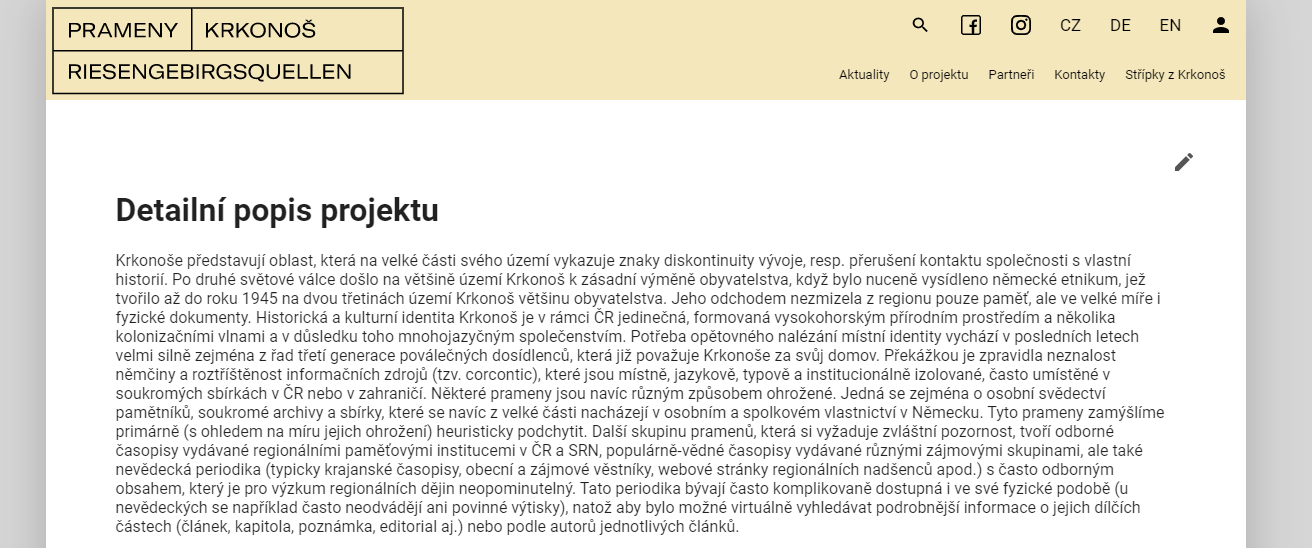
\includegraphics[width=.8\linewidth]{img/pageScene.png}
	\caption{Zobrazení normální informativní stránky}
\end{figure}

\subsubsection{Kontaktní formulář}
Pro zpětnou vazbu či otázky k projektu mohou návštěvníci využít kontaktní formulář.
\begin{figure}[H]
	\centering
	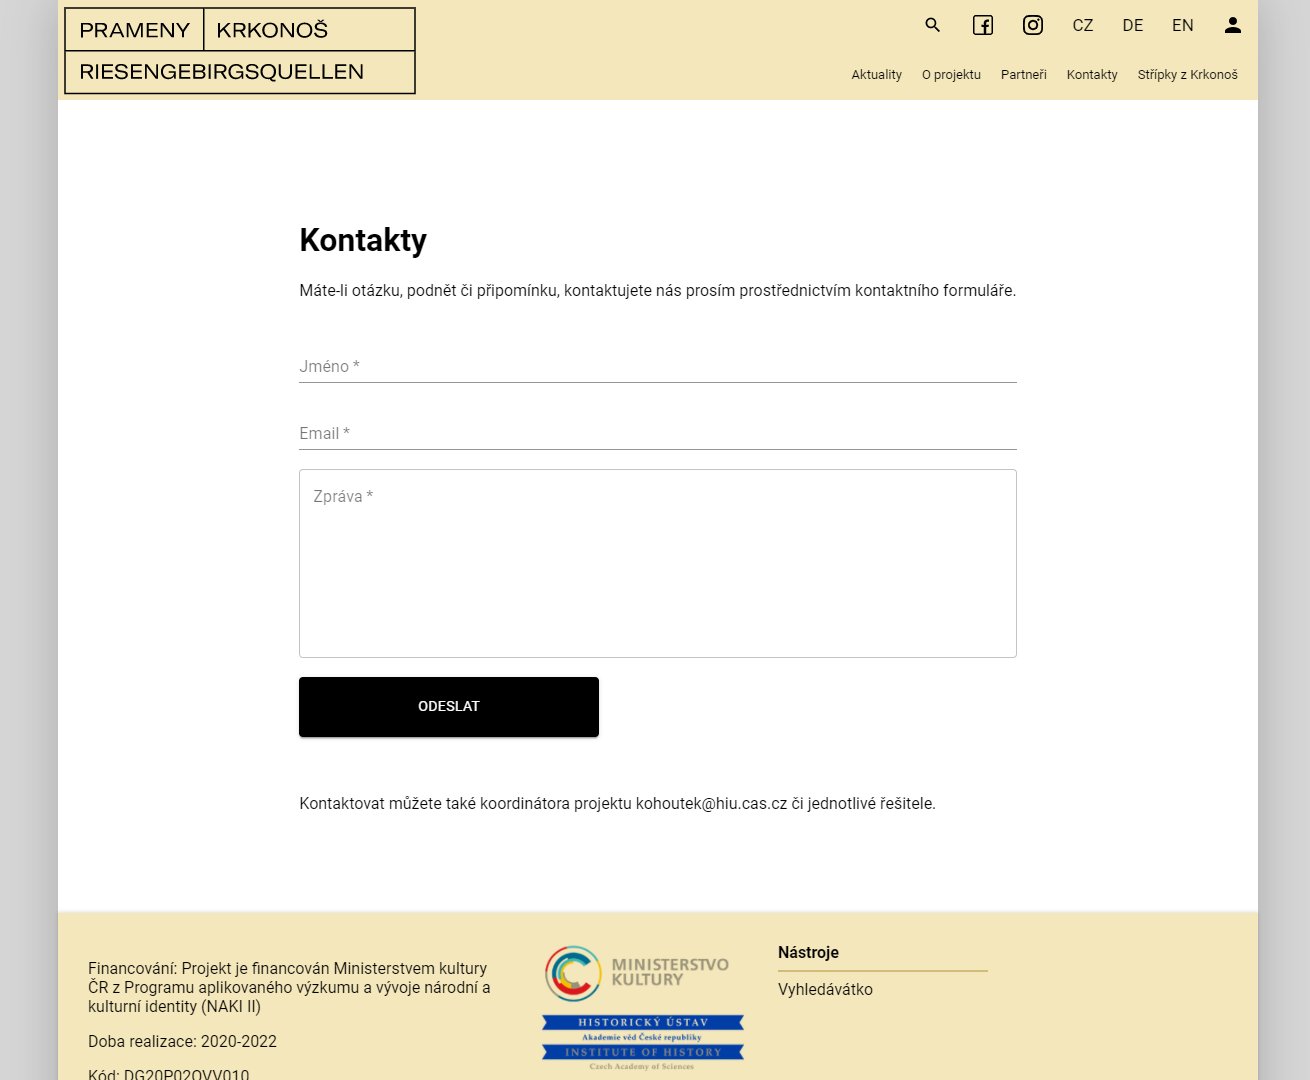
\includegraphics[width=.8\linewidth]{img/contactScene.png}
	\caption{Kontaktní formulář}
\end{figure}

\pagebreak
\subsubsection{Vyhledávátko}
Pomocí ikonky lupy v hlavičce se dostaneme do vyhledávacího prostředí.\\
Po výběru, kde chceme hledat, se nám načtou políčka k vyplnění. Uživatel do nich může zadat
libovolný výraz, a to s podporou regexp syntaxe. Ihned při vyplňování se načítá až pět
prozatím nejvhodnějších výskytů hledání. Při kliknutí na tlačítko \uv{vyhledat} se provede
vyhledání všech odpovídajících záznamů.\\
Nalezené záznamy se objevují v tabulce pod vyhledávacím polem.
Tabulka dokáže záznamy třídit po kliknutí na hlavičku příslušného sloupce.
Po kliknutí na záznam se otevře editační prostředí pro vybraný záznam.
\begin{figure}[H]
	\centering
	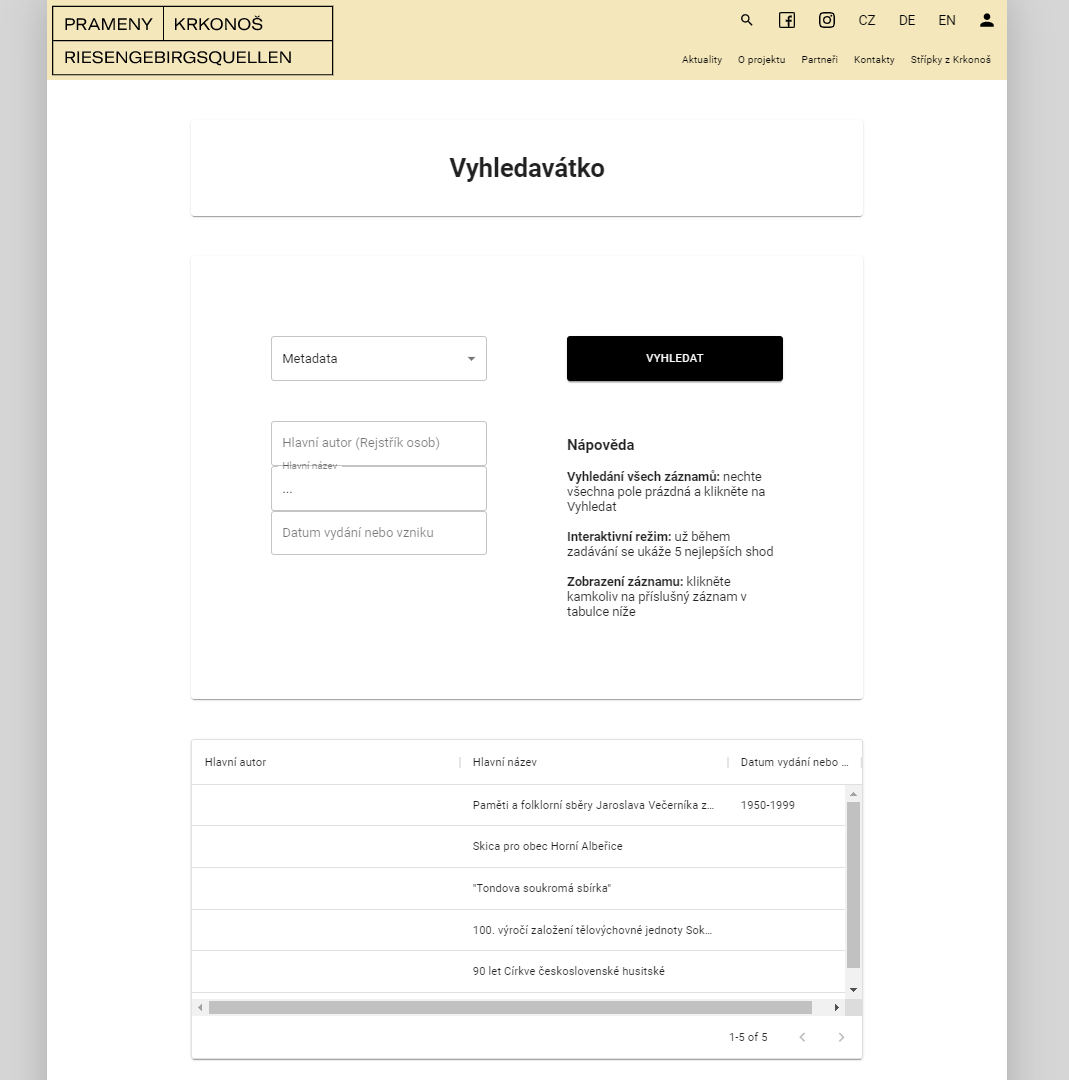
\includegraphics[width=.8\linewidth]{img/searchScene.png}
	\caption{Frontend Vyhledávátka}
\end{figure}

\pagebreak
\subsubsection{Zobrazovátko}
Záznam uložený v databázi si je možné zobrazit přes toto rozhraní, poté co
se k němu dostaneme přes vyhledávací rozhraní nebo pomocí unikátního
url linku, který se po vytvoření záznamu již nezmění.
\\
Po načtení se uživateli zobrazí záznam tak, jak je uložen v databázi, případně
s přeloženými názvy, pokud to je pomocí spodního přepínače povolené.
Dole jsou též dvě tlačítka pro smazání záznamu a editaci záznamu, jež uživatele
přesune do editačního rozhraní s aktuálním záznamem (samozřejmě jen pokud 
má dostatečná oprávnění).
\begin{figure}[H]
	\centering
	\includegraphics[width=.7\linewidth]{img/showScene.png}
	\caption{Frontend Zobrazovátka}
\end{figure}


\subsubsection{Přihlašování}
Pokud uživatel klikne na ikonku postavičky vpravo v hlavičce, nebo se pokusí dostat
na stránku, ke které nemá oprávnění, je přesměrován do přihlašovacího prostředí.
Pokud se na této stránce přihlásí, nebo již přihlášen byl, zobrazí se mu podrobnosti o jeho účtu,
včetně dostupných oprávnění.\\
\begin{figure}[H]
	\centering
	\includegraphics[width=.49\linewidth]{img/loginSceneB.png}
	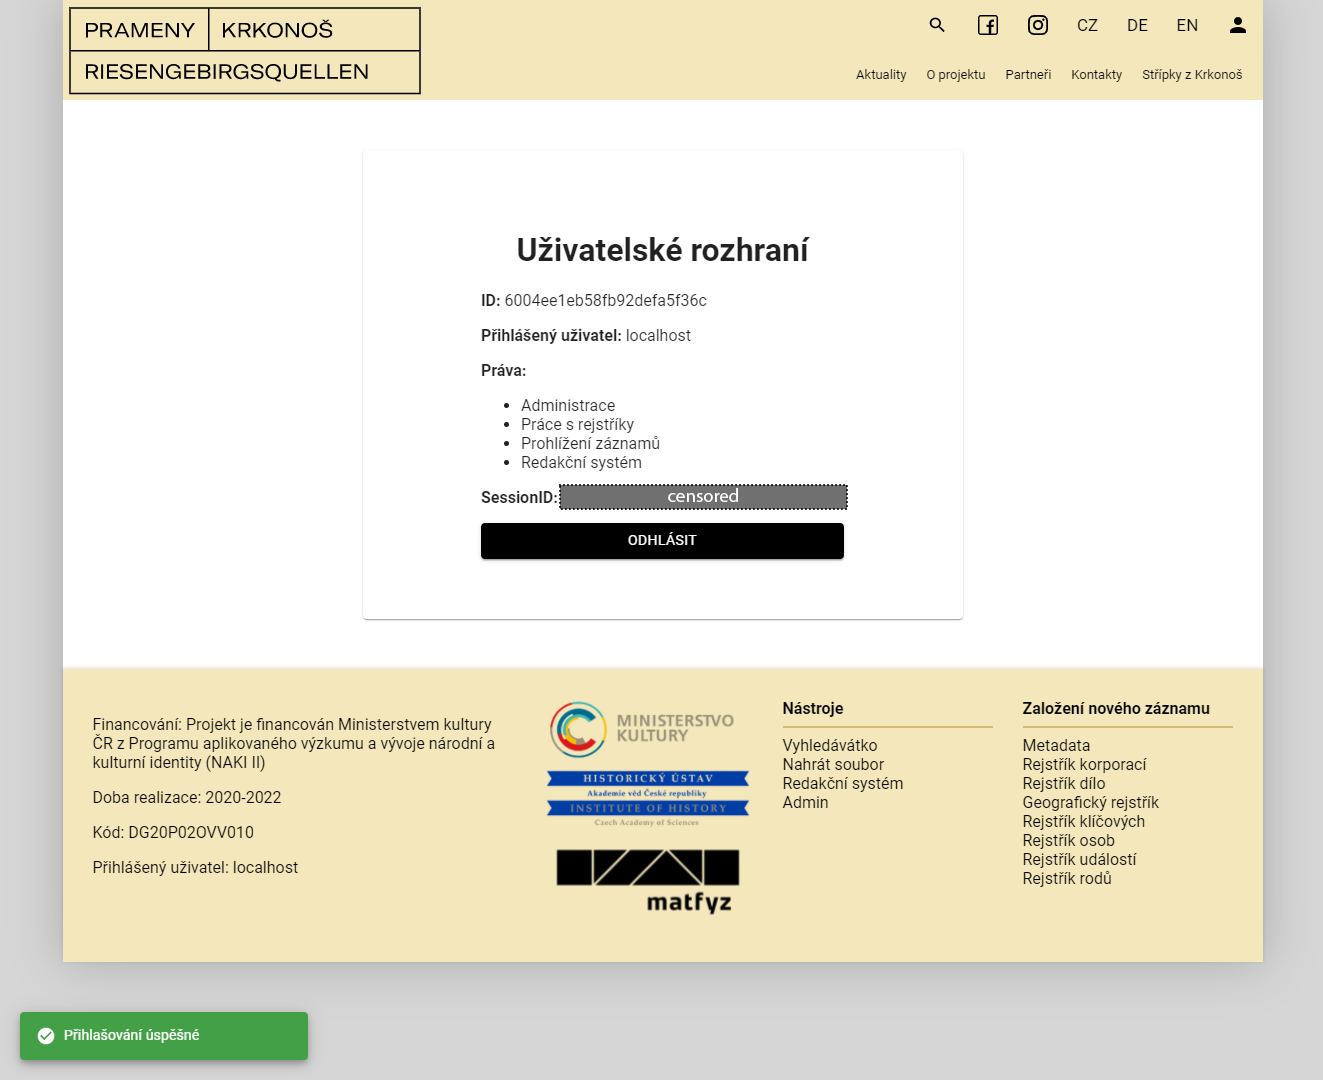
\includegraphics[width=.5\linewidth]{img/loginSceneA.png}
	\caption{Přihlašovací stránka vlevo a stránka s informacemi o přihlášeném uživateli vpravo}
\end{figure}


\subsubsection{Upravovátko}
V tomto prostředí je možné záznam upravovat a jedná se o nejkomplikovanější scénu tohoto projektu.\\
Každý typ záznamu a každý podtyp metadatové struktury má vlastní příslušná datová pole.
Ty, které umožňují mít více hodnot, mají vpravo od sebe tlačítka plus a mínus,
jehož vertikální velikost určuje velikost bloku, jež je jedním celkem. Plusové tlačítko přidává
další datové pole, zatímco mínus datové pole vyprázdní a poté odebere z náhledu.
\\
Datová pole jsou roztříděna do menších bloků a lze tlačítkem minimalizovat
(vyplněná data se nezahodí, ale pouze skryjí), aby uživateli usnadnily orientaci.
Po minimalizaci, resp. maximalizaci, bloku může dojít k převážení
sloupců a některé bloky tak mohou střídat levý a pravý sloupec, tak aby celková stránka byla co nejkratší
a prázdného místa bylo co nejméně.\\
Některé záznamy mají možnost nahrát přílohu, ta se aktivuje po kliknutí na tlačítko uploadu, s ikonkou šipky
směrem nahoru. Nahraný soubor se ihned přenáší na server a do příslušného pole automaticky 
zaznamená aktuální url nahrávaného souboru.\\
Po kliknutí na tlačítko Nahrát se buď objeví červené vyskakovací okno s chybou, proč záznam nelze uložit
(většinou zapříčiněný zadáním unikátního názvu, jež již je v databázi uložen).
Nebo se stránka znovu přepne do \textit{Zobrazovátka} a vyskočí zelené potvrzovací okénko.
\begin{figure}[H]
	\centering
	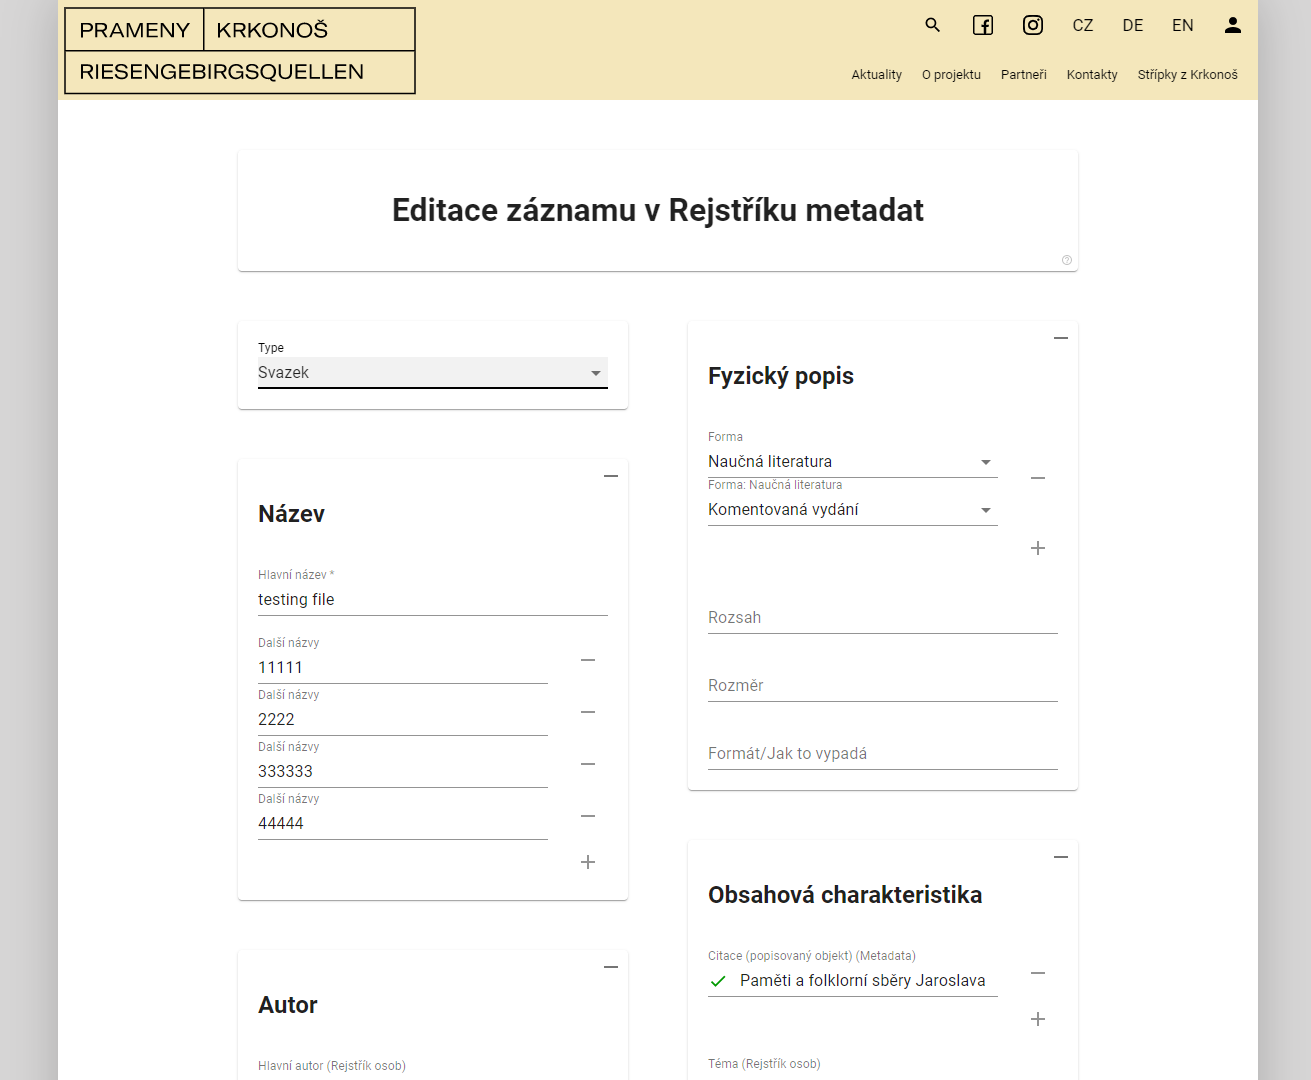
\includegraphics[width=.8\linewidth]{img/editScene.png}
	\caption{Frontend Upravovátka}
\end{figure}

\pagebreak
\subsection{Komponenty}
Komponenty jsou vlastně zapouzdřené třídy, které se dají použít vícekrát.
Každá komponenta je vhodná pro React systém a většinou je psaná bez tzv. hooků
(alternativní přístup k proměnným u komponent typu funkce, namísto typu třída).

\subsubsection{ComboBox}
\begin{wrapfigure}{r}{0.4\linewidth}
	\centering
	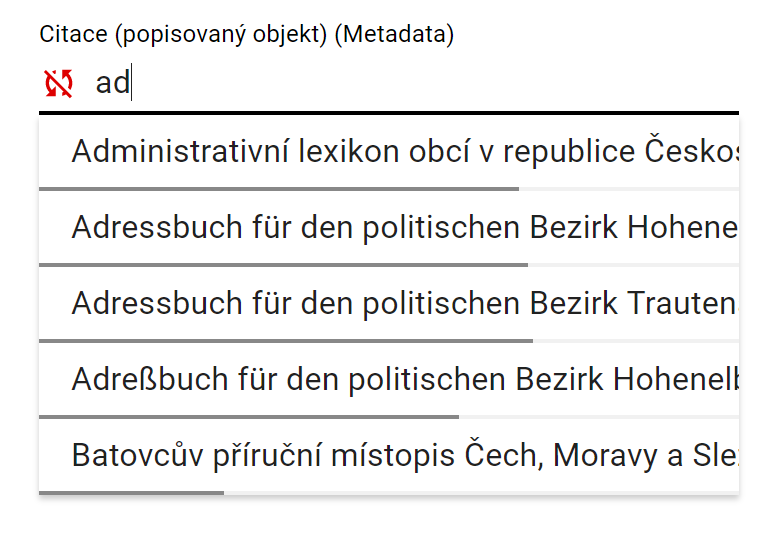
\includegraphics[width=\linewidth]{img/ComboBox.png}
	\caption{Komponenta ComboBox}
\end{wrapfigure}
ComboBox je textové pole, které při vyplňování realtime vyhledává v databázi vyhovující shody,
které zobrazuje ve formě nabídky pod tímto textovým vstupem. Po kliknutí na nabízenou položku se
do pole vyplní hodnota a na pozadí se do pole uloží ID záznamu (to se poté odesílá na server).
Dokud uživatel některý ze záznamů nevybere, pole není v konzistentním stavu a nemá možnost se
odeslat na server, což značí ikonka
\includegraphics[height=\fontcharht\font`\B]{img/notSynced.png}.
V případě, že pole má přiřazené ID záznamu a zobrazuje název, rozsvítí se ikonka
\includegraphics[height=\fontcharht\font`\B]{img/synced.png},
která značí, že data z tohoto pole se při uložení správně odešlou na server.
Popisky často bývají dlouhé, a proto je zde i miniaturní posuvník, se kterým se
dá pohodlně pracovat pomocí najetí myši na políčko, přidržení klávesy \textit{Shift} a
točením kolečka na myši.

\subsubsection{Zápatí}
Jako každá správná stránka i tato má zápatí, jež obsahuje povinné údaje o projektu a
rychlé odkazy.\\
Jelikož se jedná o projekt MK ČR - NAKI, nalezneme zde povinné údaje, kód projektu a
loga sponzora, zadavatelů a vývojářů.
Níže je ukazatel aktuálně přihlášeného uživatele.
V pravé části jsou pak rychlé odkazy, které se zobrazují v závislosti na právech přihlášeného uživatele.
Nepřihlášený uživatel tudíž v této části uvidí pouze jedno menu \uv{Nástroje} s jedinou
položkou \uv{Vyhledávátko} a po přihlášení se (viz obrázek 5.11) menu rozroste o další rychlé odkazy.
\begin{figure}[H]
	\centering
	\includegraphics[width=.8\linewidth]{img/zapati.png}
	\caption{Zápatí stránky}
\end{figure}

\pagebreak
\subsubsection{Navigační menu}
V navigačním menu nalezneme rychlé odkazy na Vyhledávátko (tlačítko s ikonkou lupy),
Facebook a Instagram projektu Prameny Krkonoš a přihlašovací stránku. Tlačítka pro
přepínání mezi třemi jazyky. Níže pak důležité stránky projektu a některé kategorie
(např. kategorie Aktuality).
\begin{figure}[H]
	\centering
	\includegraphics[width=.8\linewidth]{img/navigationBar.png}
	\caption{Navigační menu}
\end{figure}

\subsubsection{Textové pole s validací}
\begin{wrapfigure}{r}{0.4\linewidth}
	\centering
	\includegraphics[width=\linewidth]{img/validationField.png}
	\caption{Pole s kontrolou validity dat}
\end{wrapfigure}
To, že uživatel zadává data ve srozumitelném formátu (tak aby je dokázal pochopit další
uživatel, nebo aby je databáze správně interpretovala), je kontrolováno na straně klienta
(a po odeslání i na straně serveru).
V případě, že data požadovaný formát nemají, pod políčkem se zobrazí varovný nápis a
záznam nepůjde uložit, dokud všechna pole nejsou ve správném formátu.

\subsubsection{Pole pro nahrávání souborů}
\begin{wrapfigure}{r}{0.4\linewidth}
	\centering
	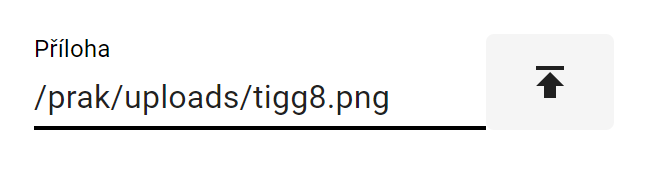
\includegraphics[width=\linewidth]{img/uploadField.png}
	\caption{Pole pro nahrávání souborů}
\end{wrapfigure}
U některých záznamů je užitečné uchovat přílohu ve formátu obrázku nebo dokumentu.\\
Tyto soubory lze nahrát na server a do databáze uložit pouze odkaz na jejich umístění,
protože databáze není stavěná na uchovávání obrázků a podobných relativně velkých souborů.

\subsubsection{Indexy}
Hlavní částí editačního rozhraní jsou indexové objekty, které určují, která pole
se mají zobrazit při různých typech záznamů. Pro každý typ je zde JSON soubor, ve kterém
je seznam polí a informace o nich. Mezi tyto informace patří především popisek, struktura, jak
data odeslat do databáze, nápověda přístupná pomocí malého otazníčku a nepovinná pole jako
požadavek na nenulovou hodnotu, nebo regexpový výraz pro kontrolu formátu dat.

\subsection{Moduly}
Funkcionalita, která není až tak často používána, se do hlavního souboru aplikace
nepřidává a tudíž čistý frontend žádné moduly nepodporuje. Moduly jsou výhradně načítány
ze serveru a neobsahují hlavní frontend.

\section{Lokalizace}
Překlad stránky do různých jazyků je řešen pomocí knihovny i18n, která je velmi efektivní a
zároveň poskytuje snadný způsob, jak texty překladu přidávat a editovat. 
Překlady navíc jsou rozloženy do více souborů a úrovní, takže se překlad velmi dobře
škáluje i na větší projekty.\\
Výsledkem jsou lokalizační soubory ve formátu JSON, které frontend aplikuje na požadovaných
místech. Pokud ovšem překlad chybí, použije se nejbližší možná interpretace, podobný jazyk nebo
zdrojová adresa překladu a vývojáři ukáže zprávu o chybějícím překladu.
\begin{figure}[H]
	\centering
	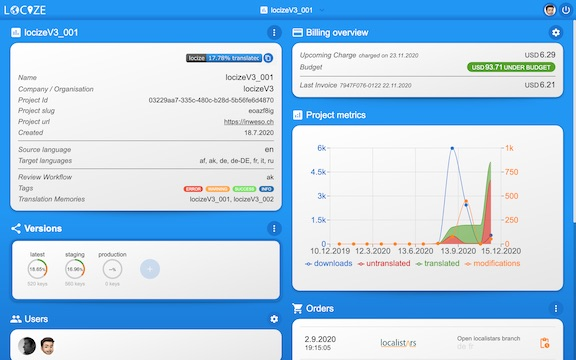
\includegraphics[width=.7\linewidth]{img/locize.jpg}
	\caption[Aplikace Locize umožňující správu překladů knihovny i18n, zdroj: \url{https://locize.com/}]{Aplikace Locize umožňující správu překladů knihovny i18n}
\end{figure}
\chapter{Provázaní Backendu a Frontendu, API}

\section{Dokumentace online}
Aktuální dokumentace, tak aby mohla být časem aktualizována a mohli do ní
být připisovány další věci, se nachází na webu
\href{http://quest.ms.mff.cuni.cz/prak/api/documentation}{.../prak/api/documentation}.
\\
Dokumentace je rozdělena na dvě části.
\\
\\
\textbf{Levá část} popisuje volání API.\\
Každá sekce tu má příslušné http metody (GET, POST atd.),
jejichž účel a formát je popsána uvnitř bloku, spolu s dalšími možnými parametry.
Spolu s formátem requestu je zde i formát odpovědi.
Podle kódu zjistíme, jestli byl náš požadavek úspěšný.
Kódy jsou standardní podle "http status codes".
\begin{itemize}
	\item \textbf{2xx} Všechno dopadlo dobře
	\item \textbf{4xx} Chyba je na straně klienta
	\item \textbf{5xx} Chyba je na straně serveru
\end{itemize}
V případě úspěchu (kód 200 - OK) se odešle odpověď na dotaz nebo
prázdné tělo, pokud request neměl za funkci něco vracet.
V případě neúspěchu pak v odpovědi najdeme zprávu o chybě, která nastala.
Obvykle to u kódu 500 bývá odeslání duplicitního záznamu.
\\
\\
\textbf{Pravá část} popisuje strukturu schémat jednotlivých modelů.\\
Jelikož databáze má datové formáty, zatímco JSON soubor ne (nebo alespoň ne tak rozsáhlé),
musí i odesílaná data mít správný formát nebo alespoň být validní po automatickém
přetypovaní.
Schéma tvoří JSON objekt, jež toto schéma popisuje.
Pokud je datový typ položky objekt buď se opravdu jedná o objekt, nebo
se jedna pouze o upřesněni datového typu.
Klíčovými slovy jsou:
\begin{itemize}
	\item \textbf{type}: datový typ
	\item \textbf{required}: true, pokud je tato položka povinná
	\item \textbf{unique}: true, pokud se zadaná hodnota nesmí shodovat s již existující položkou v DB
	\item \textbf{ref}: název schématu, na který se ID odkazuje
	\item \textbf{refPath}: speciální ref, umožnující uživateli zadat i název schématu, vůči kterému se odkazuje
\end{itemize}
Pokud je hodnota pouze string, pak je tato hodnota datovým typem.

\subsection{Software pro online dokumentaci}
Pro možnost stažení dokumentace a prohlížení offline, je vše zabaleno do jediného html souboru.
Uvnitř je zdrojový kód programu, jež vykresluje stránku a zároveň data dokumentace.
\\
Program vykresluje veškeré položky s daty dokumentace.
Bloky zdrojových kódu jsou vysázený fontem monospace a obarveny, aby uživateli
poskytly rychlejší orientaci v kódu.
\\
\begin{figure}[H]
	\centering
	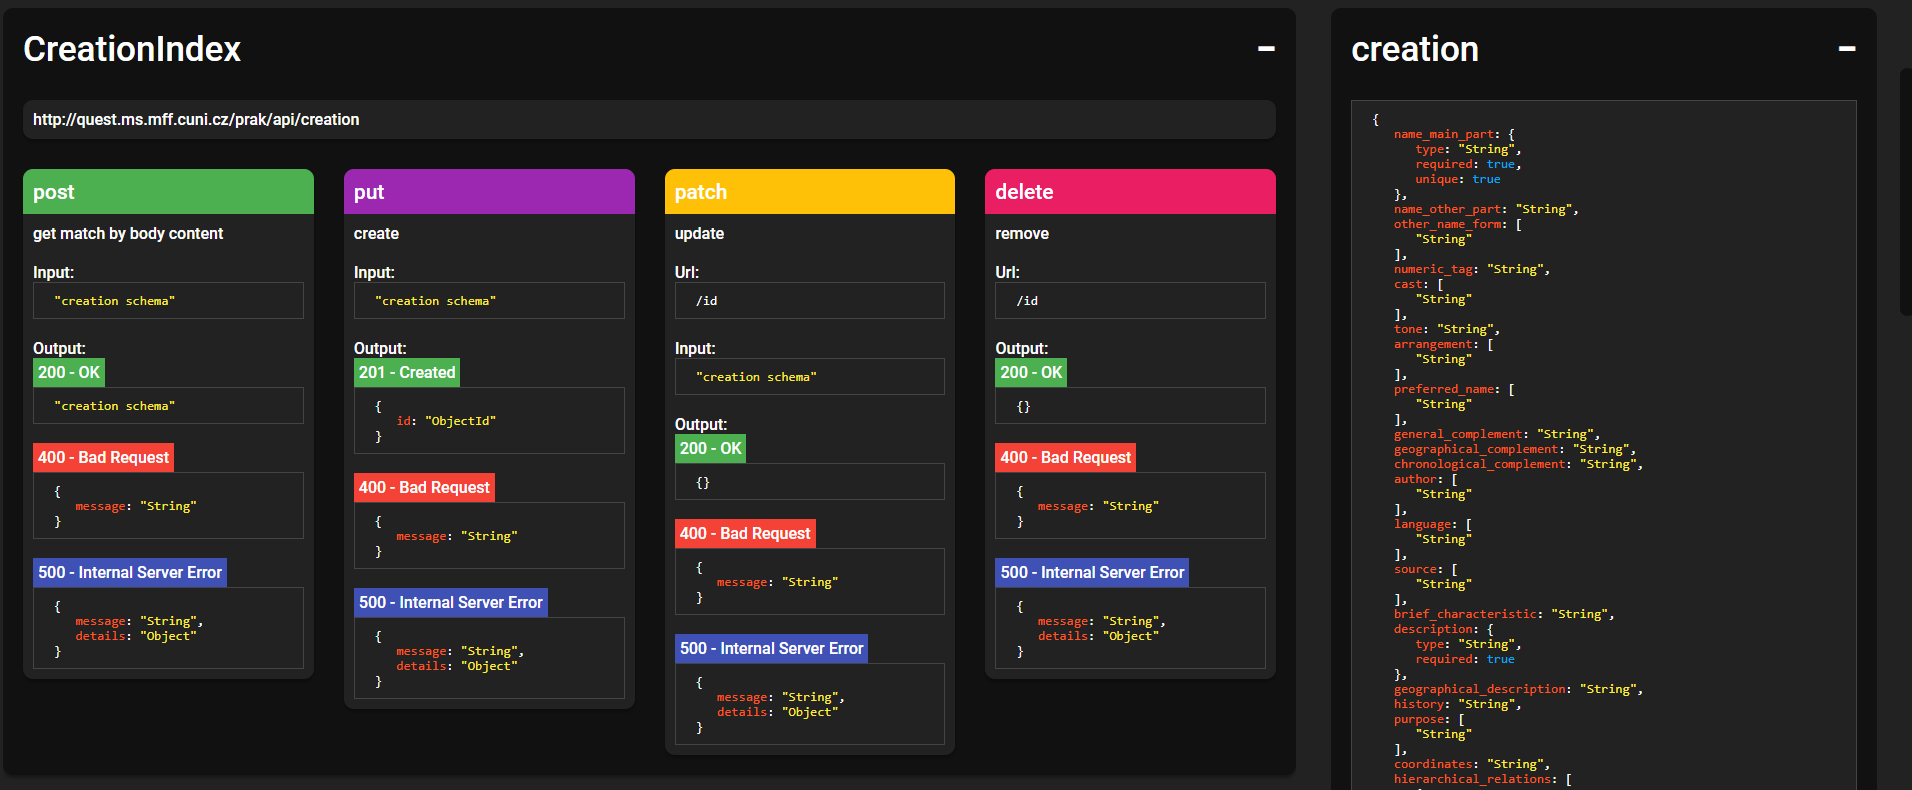
\includegraphics[width=\linewidth]{img/documentationPreview.PNG}
	\caption{Dokumentace API jako webová stránka}
\end{figure}


\section{Backend}
Na backendu je spuštěný express server (bežící pod nodejs), který
zachytává requesty s url \texttt{...prak/api/...} .
Podle cesty, jež je uvedena za /api, se request předává
příslušnému routeru. Výjimku tvoří adresa .../api/documentation, která
rovnou přeposílá soubor s dokumentaci a není tedy pro získaní dokumentace
třeba rozumět systému requestů hlouběji.
\\
\\
Při převzetí requestu jedním z mnoha routerů se porovnává
typ requestu (POST, PUT atd.) a případné detaily cesty v url.
Při plném nalezení shody se provede ověření práv, pokud je to potřeba.
Pokud request má požadovaná oprávnění, je provedena příslušná funkce
a uživateli je vrácena odpověď případně potvrzení o úspěchu.
V případě, že request nemá příslušná oprávnění, je vrácen kód 401.
V případě, že se na serveru něco pokazí, vrátí se kód 400, nebo 500, podle typu problému.

\section{API}
API je přístupné na adrese \texttt{quest.ms.mff.cuni.cz/prak/api/...} .

\subsection{Autentifikace}
S každým requestem přichází v hlavičce i cookie, ten pro
autentifikaci se jmenuje "sessionID".
Podle něj se najde příslušný uživatel a porovnají se jeho práva a
práva potřebná pro vykonání požadované funkce. Pokud jsou práva nedostatečná,
vrátí se odpověď s kódem 401, v případě správného oprávnění router vykoná funkci,
jež danému requestu přísluší, a pokud se nepokazí nic jiného, vrátí validní odpověď.

\section{Frontend a volání API}
Jelikož je celý projekt zamýšlen jako webová aplikace, nejstandardnější použití
je volání API pomocí JS funkce \textit{fetch()}, což je pouze technický alias pro XMLHttpRequest.
Ale je možné jej volat jakkoliv jinak, dokud to bude validní http request.

\subsection{Fetch}
Dokumentace metody: \href{https://developer.mozilla.org/en-US/docs/Web/API/Fetch_API}{developer.mozilla.org}
\\
Příklad použití:
\\
\begin{lstlisting}[language=JavaScript]
	const url = "/prak/api/metadata" 
	fetch(url, {
		method: "POST",
		headers: { "Content-Type": "application/json" },
		body: JSON.stringify({
			"_limit" : 100, // max returned count by default is 5 
			"name"   : "..."
		}),
	})
	.then(response => {
		if(!response.ok) throw response
		return response.json()
	})
	.then(response => {
		console.log(response)
	})
	.catch(error => {
		console.error(error)
	})
\end{lstlisting}

\subsection{Existující programy pro práci a testovaní API}
\begin{figure}[H]
	\centering
	\includegraphics[angle=90,width=.87\linewidth]{img/InsomniaExample.PNG}
	\caption{Program Insomnia s vyplněným dotazem pro odeslání požadavku na API}
\end{figure}

\chapter{Moduly}

\section{Přidávání nových modulů}
Nové moduly se nahrávají do složky \textit{modules},
která leží vedle adresářů \textit{frontend}, \textit{backend} a \textit{uploads}.
Nahrávat lze jednotlivé html soubory, složky se složitější architekturou nebo
celé npm balíčky s vlastní zkompilovanou stránkou. Moduly by měly být nezávislé na
obsahu diskového prostoru v \uv{rodiči} a měly by tedy být samostatně spustitelné,
maximálně s interakcí s API.

\section{Aktuálně nasazené moduly}

\subsection{Modul hologram}
Tento modul bude sloužit na výstavě Pramenů Krkonoš k zobrazování 3D objektů ve formě hologramu,
který se bude pomalu otáčet a ukáže se tak návštěvníkovi ze všech stran.

\subsubsection{Načítání modulu}
Tento modul obsahuje velkou knihovnu, a tudíž není efektivní jej mít v primární aplikaci.
Protože by se tyto knihovny načítaly, i když by uživatel s tímto modulem neměl v plánu pracovat.
Což většinu času nebude chtít, a tudíž by to pouze vedlo ke zpomalení systému.
Systémem \textit{Lazy} načítání je tedy celý modul odříznut a načítá se až explicitně při jeho použití.

\subsubsection{Grafický engine}
Pro vykreslování 3D modelu na webu slouží WebGL, grafická knihovna podobná staré verzi OpenGL.
Reálně jsou dostupné dvě propracované knihovny pro práci ve WebGL.
ThreeJS, které se zaměřuje na statické vykreslování a předvádění.
BabylonJS, která naopak napodobuje známé programy jako je \textit{unity} a má podporu
fyziky a dalších podknihoven užitečných pro tvorbu her.
Pokud pomineme možnost naprogramovat vše od základu, nejvhodnější knihovnou 
je \textbf{ThreeJS}.\\
Z této knihovny využijeme moduly pro načítání modelu a textury, jejich spárování a
efektu Peppers Ghost, který je implementován pomocí 4 nezávislých kamer.


\subsubsection{Peppers Ghost Effect}
\begin{figure}[H]
	\centering
	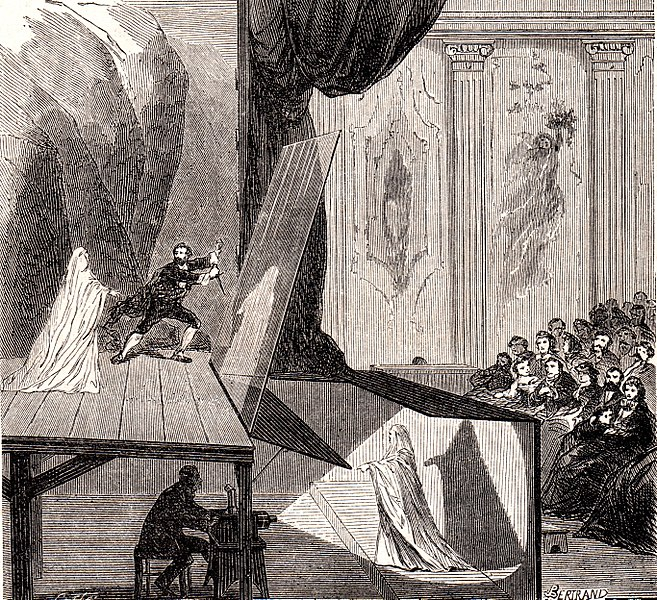
\includegraphics[width=.5\textwidth]{img/Peppers_Ghost.jpg}
	\caption[Peppers Ghost efekt - zdroj: \url{https://commons.wikimedia.org/wiki/File:Peppers_Ghost.jpg}]{Peppers Ghost efekt}
\end{figure}

Jedná se o divadelní trik, jež skládá pozorovateli dva obrazy přes sebe a vytváří iluzi
hologramu nebo ducha. Původně byl vyvinut pro divadelní představení, v moderní
době však dokáže simulovat i hologram, který známe ze sci-fi.

\subsubsection{Modely a textury}
Modely jsou z webu \url{https://3dwarehouse.sketchup.com} a
textury z webu \url{https://www.textures.com/ a https://texturehaven.com/}.\\
V programu blender pak byly tyto textury namapovány na objekt a bylo do nich
zapečeno ambient oclusion (stíny vytvořené stísněným prostorem).



\subsection{Prohlížeč map}
Dalším historickým prvkem, který bychom návštěvníkům této aplikace poskytli, jsou
2D mapy z 19. století. Uživatel si může vybrat mapu a tu si velmi podrobně
prohlížet pomocí přibližování a posouvání.

\subsubsection{Zdroj map}
Mapy byly získány od ČUZK výměnou za jejich kompletaci.
Mapu jsme totiž dostali ve formě \uv{tady máš puzzle a poslepujte si to sami}.
Každou mapu jsme tedy pečlivě zrekonstruovali, při zachování všech detailů a
historických přesností a bez jejich upravování či umělého přidávání.

\chapter{Instalace a spuštění}

\section{Prerekvizity}
Předpokládáme instalaci na operačním systému Windows 10 s následujícími 
předinstalovanými programy.
\subsection{NodeJS}
JavaScriptový interpret v nejnovější verzi lze stáhnout z oficiálního
webu \url{https://nodejs.org/}.\\
Spolu s nodejs se nám nainstaluje i příkaz \texttt{npm}, ten ihned využijeme
k nainstalování jeho lepšího \uv{dvojčete} a to sice \texttt{pnpm}, pomocí
příkazu
\begin{lstlisting}
	npm install -g pnpm
\end{lstlisting}

\subsection{MongoDB}
Databázový nástroj lze stáhnout ze stránky \url{https://www.mongodb.com},
nebo využít službu \uv{MongoDB Atlas}, což je přednastavená databáze
na serveru Googlu (nebo u Amazonu podle preference).\\
Pro snazší konfiguraci je vhodná aplikace \textit{MongoDBCompass},
poskytující oproti webové aplikaci i příkazový řádek.

\subsection{Nginx}
Webový server lze stáhnout z oficiální stránky vývojářů \url{https://www.nginx.com/}.
Konfigurační soubor pak nalezneme dle cesty instalace:\\
\texttt{.../ChocoInstallFolder/nginx-x.xx.x/conf/nginx.conf}\\
do něj vložíme naši konfiguraci serveru (přizpůsobenou vůči místu instalace)
\begin{lstlisting}[keywordstyle=\ttfamily]
	server {
		listen 80 default_server;
		server_name _;

		# React app & front-end files
		location / {
			root /var/www/naki/frontend/build/;
			rewrite ^ /index.html break;
		}
		location /static/{ root /var/www/naki/frontend/build/; }
		location /images/{ root /var/www/naki/frontend/build/; }
		location /locales/{ root /var/www/naki/frontend/build/; }
		location /public/{ root /var/www/naki/frontend/build/; }

		location /modules/{ alias /var/www/naki/modules/; }
		location /uploads/ { alias /var/www/naki/uploads/; }

		# node API reverse proxy
		location /api/ {
			proxy_pass http://localhost:50081/;
		}
	}
\end{lstlisting}


\subsection{Powershell}
Jelikož výchozí příkazová řádka od Windows má svá léta slávy za sebou, je
vhodnější používat powershell, který se syntaxí více podobá linuxovému shellu.
Pro multiplaformní účely je nejlepší jeho \uv{core} verze, kterou lze stáhnout
z github repozitáře (v README.md je odkaz) \url{https://github.com/PowerShell/PowerShell}.

\subsection{Chocolatey balík}
Pro ty, kteří znají a mají nainstalovaný balíčkovací manager \uv{chocolatey} pro Windows, 
stačí spustit tento jednoduchý kód pro snadnou instalaci.
\begin{lstlisting}
	choco install nodejs
	choco install mongodb
	choco install mongodb-compass
	choco install nginx
	choco install powershell-core
	npm install -g pnpm
\end{lstlisting}

\section{Zdrojové soubory}
Veškerá zdrojové soubory (kromě na platformě závislé konfiguraci Nginx)
jsou uloženy na GitHubu \url{https://github.com/EbrithilNogare/PraK}

\section{Instalace}
Ve složce se zdrojovými soubory spustíme následující příkazy:
\begin{lstlisting}[language=bash]
	#####   frontend npm install
	cd frontend
	npm install

	#####   frontend build
	npm run build
	
	#####   backend npm install
	cd ../backend
	npm install
	node server
\end{lstlisting}

\chapter{Řešení}

\section{Výsledný web}
Funkční web je možné si zobrazit na adrese \url{http://quest.ms.mff.cuni.cz/prak/homepage}.
Nezapomínejte, že pro zobrazení většiny stránek jsou potřeba vyšší oprávnění,
než má nepřihlášený uživatel.

\section{Uživatelská dokumentace}
\subsection{Návštěvník (nepřihlášený uživatel)}
Při vstupu na stránku se návštěvník dostává na hlavní webovou stránku,
na které si může přečíst hlavní informace o projektu nebo aktuality.\\
Obsah stránky je převážně v češtině, ale lze přepnout jazyk ovládacích prvků
pomocí tlačítek \texttt{CZ}, \texttt{DE} a \texttt{EN} vpravo nahoře.
Pro zobrazení záznamů slouží ikonka lupy v pravém horním rohu, která směruje na
vyhledávací rozhraní, ve kterém lze záznamy vyhledat (systém podporuje i regexp výrazy),
setřídit pomocí kliknutí na záhlaví požadovaného sloupce a následně požadovaný záznam i 
zobrazit v jeho detailní podobě.\\
V hlavním menu najdeme i několik odkazů na stránky s relevantními informacemi a
rubriky jako jsou \textit{Novinky} nebo \textit{Střípky z Krkonoš}.\\
Trochu schované jsou pak odkazy na moduly:
\begin{itemize}
	\item 3D model hologram \\
		\url{http://quest.ms.mff.cuni.cz/prak/modules/hologram/}
	\item 2D mapa Krkonoš 19. století \\
		\url{http://quest.ms.mff.cuni.cz/prak/maps}
\end{itemize}

\subsection{Zadavatel}
Zadavatel se stejně jako uživatel dokáže dostat k zobrazení detailu záznamu, navíc zde má
ale i tlačítko pro editaci záznamu, jež jej přesune do editačního rozhraní.
Zde může vyplňovat pole a následně záznam uložit. Specifikace atypických polí
je v kapitole 5.3.2.\\
K vytvoření nového záznamu má zadavatel v patičce webu připraveny odkazy do
scény \textit{Zadávátka}, které je identické se vzhledem editačního prostředí.\\
V případě potřeby může zadavatel nahrát soubor na server pomocí odkazu v
patičce webu s názvem \textit{Nahrát soubor}. Po kliknutí na tlačítko
s ikonkou šipky se mu zobrazí okno pro zvolení souboru a po jeho vybrání se
soubor odešle na server a uživateli se zobrazí přímý odkaz na nahraný soubor, který
může začít ihned používat.

\subsection{Redaktor}
Pro přístup do redakčního systému stránky stačí v jejím pravém rohu kliknout
na ikonku tužky (viz \textit{Obr. 5.4}) nebo použít odkaz \textit{Redakční systém}
v zápatí stránky, kde se mu zobrazí veškeré stránky webu a odtud si může vybrat,
kterou chce editovat. Po kliknutí na ikonku oka stránku zobrazí, případně po
kliknutí na ikonku tužky ji začne editovat. Měnit lze vše kromě již existující
url. Více o redakčním systému v \textit{kapitole 5.3.1 - CMS}.


\subsection{Admin}
Veškerá správa uživatelů, jejich informací a oprávnění spadá pod administrační rozhraní,
přístupné přes odkaz \textit{Admin} v zápatí stránky.\\
Nového uživatele lze přidat v horní části administračního rozhraní, kam se
zadají potřebné údaje a uživatel se uloží. Níže pak nalezneme seznam uživatelů a
informace o nich, včetně možnosti změny jejich údajů a nebo smazání jejich účtů.

\section{Co by se dalo vylepšit a přidat}
Velké knihovní systémy mají velkou řadu funkcí pro práci nad daty, jako jsou
např. \textbf{hromadné úpravy} nebo práce se \textbf{šablonami}. Ty ačkoliv
nejsou aktuálně implementovány, tak je lze snadno vytvořit díky
dobře vytvořenému API.\\
Další vylepšení by se dalo udělat pro data v záznamu, ačkoliv databáze
je připravená v záznamu uchovat a vrátit cokoliv v jakémkoliv formátu,
tak na frontendu je nutný zásah programátora, aby přidal pole, bylo by
uživatelsky přívětivější, aby pole mohl přidávat i obyčejný zadavatel
přes \uv{klikací rozhraní}.


\chapter*{Závěr}
\addcontentsline{toc}{chapter}{Závěr}

Předmětem této práce byl návrh a vývoj softwarového řešení pro tématický
digitální archiv. týkající se sběru, uchování a prezentaci dokumentů z oblasti
Krkonoš. Výsledné softwarové řešení mělo agregovat databázi pro ukládání různých
typů dokumentů (resp. objektů) a web pro prezentaci a úpravu těchto dat. - Přičemž
rozhraní pro popis a evidenci dokumentů měl být navržen
tak, aby byla oddělena vrstva pro běžné prohlížení dokumentů, vkládání záznamů o
dokumentech a vrstva (prostředí) pro správu a editaci těchto záznamů.
Navrhovaný software měl zohledňovat typologii dokumentů a zároveň reflektovat
různé (oborové) normy pro bibliografický popis dokumentů. Při návrhu vkládacího
modulu bylo třeba zohlednit normy knihovnické, muzejní i archivní. V tomto směru
navržený software disponuje velkou inovativností v přístupu k popisu dokumentů.
Zároveň bylo třeba při návrhu software (a jeho jednotlivých modulů)
zohlednit požadavek historiků na vzájemnou provázanost jednotlivých vložených
údajů. - Tj. vytvořit takovou strukturu vkládaných záznamů, aby mezi
bibliografickými údaji a rejstříky bylo možné z různých polí vzájemně odkazovat
na jiná pole, resp. aby bylo možno odkazovat mezi bibliografickým záznamem a
rejstříkem, a taktéž mezi rejstříky navzájem.
\\

Výsledkem je webové rozhraní a serverová aplikace poskytující API pro komunikaci
s jednotlivými moduly výsledného software. V práci je popsána jak implementace
backendu, tak i implementace frontendu, ale i jejich vzájemné provázání
prostřednictvím API. Dále jsou v práci popsány další přídavné moduly k
výslednému software.
\\

Vedle hlavní frontend aplikace je možné si načíst i oddělené moduly.
První modul poskytuje hologram 3D modelu, který se hodí zejména na výstavy.
Druhý modul přináší interaktivní prohlížení 2D map z Krkonoš 19. století.
\\


Serverová aplikace poskytuje nejen samotnou webovou aplikaci, ale i
moduly nezávislé na hlavní aplikaci. Ty pak komunikují se serverem pomocí API,
které je dobře zdokumentováno a poskytuje tak přístup k datům i pro
externí programátory a jejich programy.
\\


Beta verze systému byla testována reálnými uživateli a bylo do ní
zadáno přes 35000 záznamů různých typů a velikostí.
\\

Během vývoje betaverze byl software testován \uv{ostrými} daty. Do systému bylo
uživateli zadáno přes 35 000 záznamů různých typů, velikostí či úrovně
kompletnosti. Na základě poznatků od uživatelů byl software laděn směrem k tomu,
aby rozhraní pro vkládání dat a pro jejich editaci bylo uživatelsky co
nejpřívětivější a co nejintuitivnější.
\\


%%% Seznam použité literatury
%%% Seznam použité literatury (bibliografie)
%%%
%%% Pro vytváření bibliografie používáme bibTeX. Ten zpracovává
%%% citace v textu (např. makro \cite{...}) a vyhledává k nim literaturu
%%% v souboru literatura.bib.
%%%
%%% Příkaz \bibliographystyle určuje, jakým stylem budou citovány odkazy
%%% v textu. V závorce je název zvoleného souboru .bst. Styly plainnat
%%% a unsrt jsou standardní součástí latexových distribucí. Styl czplainnat
%%% je dodáván s touto šablonou a bibTeX ho hledá v aktuálním adresáři.

\bibliographystyle{czplainnat}    %% Autor (rok) s českými spojkami
% \bibliographystyle{plainnat}    %% Autor (rok) s anglickými spojkami
% \bibliographystyle{unsrt}       %% [číslo]

\renewcommand{\bibname}{Seznam použité literatury}

%%% Vytvoření seznamu literatury. Pozor, pokud jste necitovali ani jednu
%%% položku, seznam se automaticky vynechá.

\bibliography{literatura}
\nocite{*}					% bibtex si nebude stěžovat na chybějící citace 


%%% Kdybyste chtěli bibliografii vytvářet ručně (bez bibTeXu), lze to udělat
%%% následovně. V takovém případě se řiďte normou ISO 690 a zvyklostmi v oboru.

% \begin{thebibliography}{99}
%
% \bibitem{lamport94}
%   {\sc Lamport,} Leslie.
%   \emph{\LaTeX: A Document Preparation System}.
%   2. vydání.
%   Massachusetts: Addison Wesley, 1994.
%   ISBN 0-201-52983-1.
%
% \end{thebibliography}


%%% Obrázky v bakalářské práci
%%% (pokud jich je malé množství, obvykle není třeba seznam uvádět)
\listoffigures

%%% Tabulky v bakalářské práci (opět nemusí být nutné uvádět)
%%% U matematických prací může být lepší přemístit seznam tabulek na začátek práce.
% \listoftables

%%% Použité zkratky v bakalářské práci (opět nemusí být nutné uvádět)
%%% U matematických prací může být lepší přemístit seznam zkratek na začátek práce.
\chapwithtoc{Seznam použitých zkratek}

\subsection*{Administrativní}
\begin{tabular}{| c | c |}
	\hline
		MK ČR - NAKI & Ministerstvo kultury ČR - Národní Kulturní Identita \\
	\hline
		ČUZK & Český úřad zeměměřický a katastrální \\
	\hline
\end{tabular}

\subsection*{Programátorské}
\begin{tabular}{| c | c |}
	\hline
		API & Application Programming Interface \\
	\hline
		Regexp & \makecell{Regular expression, více zde:\\\url{https://en.wikipedia.org/wiki/Regular_expression}} \\
	\hline
	DB & Databáze \\
	\hline
	cors & \makecell{Cross-origin Resource Sharing,\\soubor pravidel pro komunikaci\\napříč rozdílnými doménami}\\
	\hline
	md5 & \makecell{message-digest algorithm,\\rodina hašovacích funkcí v kryptografii} \\
	\hline
	WYSIWYG & \makecell{What you see is what you get,\\neboli \uv{co vidíš, to dostaneš}} \\
	\hline
\end{tabular}

%%% Přílohy k bakalářské práci, existují-li. Každá příloha musí být alespoň jednou
%%% odkazována z vlastního textu práce. Přílohy se číslují.
%%%
%%% Do tištěné verze se spíše hodí přílohy, které lze číst a prohlížet (dodatečné
%%% tabulky a grafy, různé textové doplňky, ukázky výstupů z počítačových programů,
%%% apod.). Do elektronické verze se hodí přílohy, které budou spíše používány
%%% v elektronické podobě než čteny (zdrojové kódy programů, datové soubory,
%%% interaktivní grafy apod.). Elektronické přílohy se nahrávají do SISu a lze
%%% je také do práce vložit na CD/DVD. Povolené formáty souborů specifikuje
%%% opatření rektora č. 72/2017.
%\appendix
%\chapter{Přílohy}
%\section{První příloha}
%
%\section{Druhá příloha}
%
%\section{Třetí příloha}
%

\openright
\end{document}
